\documentclass[12pt]{extarticle}
\usepackage[utf8]{inputenc}
\usepackage{graphicx}
\usepackage{fancyhdr}
\usepackage{geometry}
\usepackage{lipsum}
\usepackage{tocloft} 
\usepackage{hyperref}
\usepackage{amsmath}
\numberwithin{equation}{section}
\setlength{\jot}{14pt}
\usepackage{amssymb}
\usepackage{float}

\usepackage{caption}
\usepackage{pifont}
\usepackage{listings}
\usepackage{hyperref}
\usepackage{algpseudocode}
\usepackage{algorithm}
\usepackage{booktabs}
\usepackage{multirow}

\renewcommand{\tableautorefname}{Table}
\renewcommand{\figureautorefname}{Figure}
\renewcommand{\equationautorefname}{Equation}
\renewcommand{\lstlistingname}{Algorithm}
\newcommand{\algorithmautorefname}{Algorithm}

\usepackage{listings}
\usepackage{xcolor}
\lstset{
  language=Python,
  basicstyle=\ttfamily\scriptsize,
  keywordstyle=\color{blue},
  stringstyle=\color{teal},
  commentstyle=\color{gray}\itshape,
  numbers=left,
  numberstyle=\tiny,
  frame=none,
  captionpos=b,
  breaklines=true,
  showstringspaces=false
  }

\geometry{top=2.5cm, bottom=4cm, left=2.5cm, right=2.5cm}

\begin{document}

\begin{titlepage}
    \centering
    
\includegraphics[width=0.35\textwidth]{images/Logo_comillas.png}\\[1cm] 
    {\Huge \textbf{GRADO EN INGENIERÍA}}\\[0.3cm]
    {\Huge \textbf{MATEMÁTICA E INTELIGENCIA}}\\[0.5cm]
    {\Huge \textbf{ARTIFICIAL}}\\[1.5cm]
    {\Huge \textbf{TRABAJO FIN DE GRADO}}\\[1.3cm]
    {\huge INTERPRETING NEURAL NETWORKS -}\\[0.4cm]
    {\huge DEVELOPING A METHODOLOGY FOR }\\[0.4cm]
    {\huge BANKING CASE STUDIES USING }\\[0.4cm]
    {\huge EXPLAINABLE AI}\\[0.4cm]
    \textbf{Autor: Javier Prieto Domínguez}\\[0.5cm]
    \textbf{Co-Director: David Alfaya Sanchez}\\[0.5cm]
    \textbf{Co-Director: Jaime Pizarroso Gonzalo}\\
    \raisebox {-2cm}[0cm][0cm]{\large Madrid, Junio}
    \vfill
\end{titlepage}

\setlength{\headheight}{2cm}

% Configuración del encabezado
\pagestyle{fancy}
\fancyhf{}
\fancyhead[L]{
\includegraphics[width=2cm]{images/Color_logo_comillas.png}} 

\fancyhead[C]{
    \hspace{2cm}
    \textbf{UNIVERSIDAD PONTIFICIA COMILLAS}\\
    \hspace{2cm}
    Escuela Técnica Superior de Ingeniería (ICAI)\\
    \hspace{2cm}
    Grado en Ingeniería Matemática e Inteligencia Artificial
}

\newpage

{\fontsize{14}{18}\selectfont
    Declaro, bajo mi responsabilidad, que el Proyecto presentado con el título \textbf{Interpreting Neural Networks - Developing a Methodology for Banking Case Studies Using Explainable AI} en la ETS de Ingeniería - ICAI de la Universidad Pontificia Comillas en el curso académico 2024/25 es de mi autoría, original e inédito y no ha sido presentado con anterioridad a otros efectos. \\
    
    El Proyecto no es plagio de otro, ni total ni parcialmente y la información que ha sido tomada de otros documentos está debidamente referenciada.
    
    \vspace{2cm}
    
    \makebox[\textwidth][s]{Fdo.: \textbf{Javier Prieto Domínguez} \hfill Fecha: 10/06/2025}

    
    \vspace{2cm}
    
    \begin{center}
        Autorizada la entrega del proyecto \\
        \vspace{1cm}
        \textbf{LOS DIRECTORES DEL PROYECTO}
    \end{center}
    
    \vspace{1cm}
    
    \makebox[\textwidth][s]{Fdo.: \textbf{David Alfaya Sánchez} \hfill Fecha: 10/06/2025}
    \makebox[\textwidth][s]{Fdo.: \textbf{Jaime Pizarroso Gonzalo} \hfill Fecha: 10/06/2025}
}

\newpage

{\fontsize{17}{20}
    \begin{center}
        {\large A mi familia, a Miguel y Jorge, a Lucía, y a D. Alfaya por su apoyo en todo el proyecto.}
        
    \end{center}
}

\newpage
\begin{abstract}
Neural networks are increasingly employed in the banking sector for tasks ranging from credit scoring to fraud detection. Despite their powerful predictive capabilities, the opacity of neural network models poses significant challenges to their interpretability. This project aims to bridge the gap between neural network architectures and their practical interpretation by developing an innovative counterfactual method. Using Lagrange multipliers and Newton's method for optimization, we provide the minimal changes needed to modify a model's classification output for a certain instance. The proposed method fulfills most of the desired properties in counterfactual explanations, highlighting similarity, diversity, and actionability, where, through a set of weights, users can encode their real-life difficulty to change some features, tailoring the explanation given to the specific needs of every profile.\\
\\
\textbf{Keywords}: Counterfactual explanations; Interpretability; Neural networks; Lagrange multipliers; Newton optimization; Actionability; 
\\
\\
\\
\\
\\
Las redes neuronales se emplean cada vez más en el sector bancario para tareas que van desde la concesión de crédito hasta la detección de fraude. Pese a su gran capacidad predictiva, la opacidad de estos modelos plantea serios retos de interpretabilidad. Este proyecto pretende salvar la distancia entre la potencia de las redes neuronales y su comprensión práctica mediante el desarrollo de un método contrafactual innovador. Utilizando multiplicadores de Lagrange y el método de Newton para la optimización, identificamos los cambios mínimos necesarios para modificar la salida de clasificación de un modelo en un caso concreto. El método propuesto satisface la mayoría de las propiedades deseables en las explicaciones contrafactuales, destacando la similitud, la diversidad y la accionabilidad: a través de un vector de pesos, los usuarios pueden codificar la dificultad real de alterar cada característica y personalizar así la explicación a las necesidades de cada perfil.\\
\\
\textbf{Palabras Clave}: Explicaciones contrafactuales; Interpretabilidad; Redes neuronales; Multiplicadores de Lagrange; Optimización de Newton; Accionabilidad;

    % \textcolor{red}{Un abstract demasiado abstracto. Aterrizalo un poco con cual es tu objetivo, como lo buscas, y un resumen de resultados}
\end{abstract}

\newpage
\tableofcontents
\thispagestyle{fancy}


\newpage

\section*{Introduction}
Many entities like banks face two challenges when it comes to regulations in the AI field. Regulations such as the EU GDPR require institutions to \emph{explain} model outputs used for business decisions. Classic scoring engines (logistic regression, decision trees) used now are interpretable, but often underperform modern neural networks.

Our goal is to bridge performance and interpretability by creating a \emph{counterfactual explanations} method. These methods are part of the eXplicable Artificial Intelligence (XAI) field, and they are used to explain what is the change needed to flip a model's decision for a given instance. For example, if a loan application is rejected, the method should suggest actionable changes to the applicant's profile that would change the decision to be approved. 
\begin{figure}[H]
    \centering
    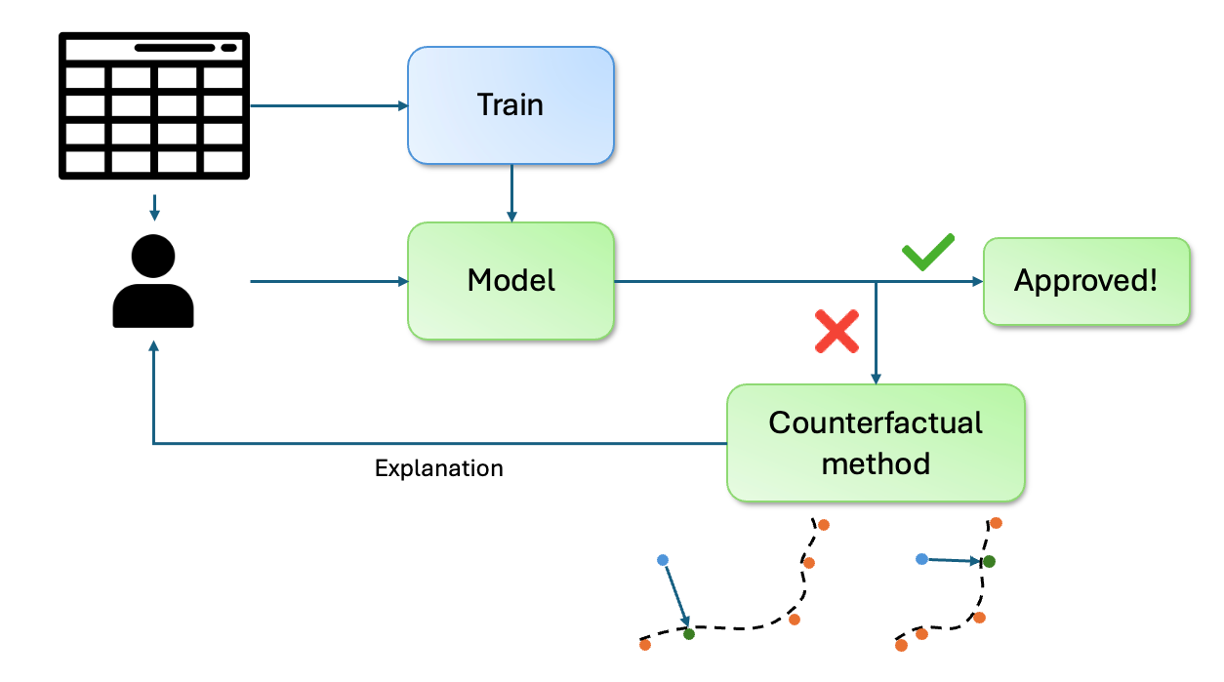
\includegraphics[width=0.4\textwidth]{images/diagram}
    \caption{Counterfactual model architecture}
    \label{fig:architecture}
\end{figure}


\section*{Related Work}
The field of Counterfactual Explainations has been around for a while, with many methods proposed to tackle the problem of explaining neural networks. Not all methods are have the same properties, and often is difficult to choose the one suitable for a given use case. For that, ~\cite{guidotti2024counterfactual} proposes a set of properties a good counterfactual explanation should fulfill, such as \emph{validity, similarity, plausibility, actionability, diversity, efficiency,} and \emph{stability}. Some methods like WACH~\cite{wachter2017counterfactual}, ACTREC~\cite{ustun2019actionable}, DiCE~\cite{dice} and SGNCE~\cite{sgnce} have been proposed to tackle the problem of counterfactual explanations, but they do not fulfill all the properties mentioned above. 

In this project, we propose an innovative method based on mathematical optimization that uses second-order derivatives to find the optimal solution to the problem, ensuring most of the properties and establishing a baseline for future work, where the method can be improved to fulfill all of them.

\section*{Methodology}
The method we propose formulates the counterfactual generation using Lagrangian multipliers. Given an instance $\mathbf{x}\! \in\! \mathbb{R}^m$, a differentiable classifier $M$, and a decision threshold $\varepsilon$, we seek to solve the optimization problem defined as
\begin{equation}
\label{eq:lagrangian_eqn}
\mathcal{L}(\mathbf{x}, \lambda) = \; C(\mathbf{x}) + \lambda \, \Bigl(M(\mathbf{x}) - \varepsilon \Bigr)
\end{equation}

where $C$ is a \emph{weighted} $\ell_2$ cost $C(\mathbf{x}) = \sum_{i=1}^m w_i\bigl(x_i - x_{0,i}\bigr)^2$. The weights, editable by the entity or end-user, encode the relative effort, or cost, of changing each feature $x_i$ from its original value. If the weight for a feature is high, it means that changing that feature is difficult or costly, while a low weight means that changing that feature is easy or cheap. This is the key part of the method, as it allows for flexibility, customization and actionability. 

To solve equation \ref{eq:lagrangian_eqn}, we need to find the minimum of the Lagrangian function $\mathcal{L}$, i.e., finding the values that satisfy $\nabla \mathcal{L}(\mathbf{x}, \lambda) = 0$, where the system of equations is given by
\[
F(\mathbf{x}, \lambda) \;=\; \nabla \mathcal{L}(\mathbf{x}, \lambda) \;=\; 0:
\begin{cases}
\nabla C(\mathbf{x}) \;-\;\lambda \cdot \bigl(\nabla M(\mathbf{x})\bigr) \;=\; 0 \\
-\,M(\mathbf{x})\;+\;\varepsilon\;=\;0
\end{cases}
\]
This is solved via a pseudo-Newton iteration that leverages \textbf{second-order} derivatives to find the roots of $F$. The normal update step is given by
\[
\bigl(\mathbf{x}_{n+1},\,\lambda_{n+1}\bigr)
\;=\;
\bigl(\mathbf{x}_n,\,\lambda_n\bigr)
\;-\;
\mathbf{H}^{-1}\!\bigl(\mathcal{L}(\mathbf{x}_n,\lambda_n)\bigr)
\;\cdot\;
\nabla\mathcal{L}\bigl(\mathbf{x}_n,\lambda_n\bigr).
\]
As we are using the inverse of the hessian matrix, ill-conditioned Hessians might make the previous step unfeasible to calculate. To mitigate this, we implement an alternative update step that uses the normalized gradient of the model's output with respect to the input features to update even when the Hessian is ill-conditioned:

\[
    \mathbf{x}_{n+1} = \mathbf{x}_n - \frac{\nabla M(\mathbf{x_n})}{|\nabla M(\mathbf{x_n})|};\;
    \lambda_{n+1} = \lambda_n
\]

\subsection*{Handling discrete features}
The previous equations assume that all input variables are continuous. However, not all input variables are numeric in real datasets. For example, if the number of credit lines is used as an input variable %\textcolor{red}{pensar otro ejemplo}
, it cannot take a decimal value. An adaptive regularizer is needed to force the input variable to collapse to an integer value:
\[
R(\mathbf{x})=\sum_{i:\, x_i\in \mathcal{Z}}\bigl(x_i-\lfloor x_i\rceil\bigr)^2
\]
This regularizer is injected into $C$ only when the iterate is near the optimal solution, forcing integer-valued features towards \emph{legal} values. Categorical features are one-hot encoded, but we have not yet implemented a way to handle them in the method.

\section*{Empirical Evaluation}
To evaluate we use different datasets~\cite{kaggleLoan1,spambase,santander} ranging from 8 to 200 features. The metrics we evaluate are: validity, similarity, plausibility, efficiency, stability, and actionability.
%\textcolor{red}{Los siguientes párrafos, mételos en un itemize}
\begin{enumerate}
    \item \textbf{Validity \& Similarity.} Newton's algorithm finds the minimal change needed to change the model's classification output for a specific sample. 
    \item \textbf{Plausibility.} $100\%$ of generated explanations were in-bounds of the original dataset and non-outlying.  
    \item \textbf{Efficiency.} Runtime varying between $0.02$-$0.16$ in the datasets used, $\sim10x$ faster than DiCE~\cite{dice} and more than $100x$ faster than SGNCE~\cite{sgnce}
    \item \textbf{Stability.} Counterfactual distance ratios $\approx0.8$–$1.0$, showing stable results.
    \item \textbf{Actionability.} We let the user to define the weights, encoding the difficulty to change each feature, allowing for diverse and realistic counterfactuals.
\end{enumerate}

% The method proposed in this work correctly generates counterfactuals that are valid and successfully finds the minimal change needed to flip the model's decision, fulfilling the similarity property as well. We measure plausibility with two main metrics. We evaluate if the counterfactuals are within the empirical bounds of the original dataset, and we also use the Local Outlier Factor (LOF)~\cite{lof} to measure if they are in-distribution. All of these criteria are met by all of the samples in out test set, composed of 176 instances of each dataset. 

% In the field of efficiency, we measure the time it takes to generate a counterfactual for each instance. Our method takes around 0.02 seconds for 8 features and around 0.16 seconds for 200 features, which is around 10 times faster than DiCE~\cite{dice} and more than 100x faster than SGNCE. In stability we obtain distance ratios of around 0.8 to 1.0 across $20$-nearest neighbors, meaning that the method yields similar counterfactuals for similar initial instances. Actionability is one of our biggest contributions, as we allow the user to set the weights for each feature, which allows for a wide range of counterfactuals to be generated. As the property is defined as how realistic are the changes proposed, and the user can set the weights to determine how easy or difficult it is to change each feature, we revolutionize the definition.

\section*{Web Application}
A lightweight \texttt{streamlit} website showcases the model's capabilities, allowing users to interactively generate counterfactuals. This is a customizable web that works with any dataset and consists of a form in which the client/user introduces their personal data and the set of weights they want to use. If the model outputs a negative classification for the data introduced, the website will generate the counterfactual and tell the user the changes they should make to flip the model's decision. The code to reproduce this website can be found here: \url{https://github.com/javiprietod/TFG}

\section*{Conclusions and Future Work} 

%\textcolor{red}{Reescribir este párrafo, que esté basado en Newton no es lo importante si no lo que consigues con el método y las ventajas que tiene comparado con otros métodos}

This work presents the first counterfactual explanation algorithm whose search procedure is entirely grounded in Newton optimization. A weight vector inside the cost function encodes how hard it is in real life to modify each feature, so analysts or end-users can rule certain attributes immutable (e.g., age) or make others cheap to change. This innovative codification of reality has not yet been found in any method in the literature.

Future work targets four extensions: (1) adding a sparsity regularizer to minimize the number of changed features, balancing similarity versus minimality; (2) learning an informed initial weight vector from logged user feedback so the system starts with feature costs that historically yielded the most actionable counterfactuals; (3) expanding the method to work with one-hot encoded categorical features; and (4) working with business stakeholders to deploy our solution in real world scenarios. Together, these directions aim to personalize explanations further and broaden dataset compatibility.

\newpage

\section*{Introducción}
Muchas entidades, como los bancos, se enfrentan a dos desafíos en lo que respecta a la regulación del uso de la IA. Normativas como el GDPR Europeo exigen a las instituciones \emph{explicar} las salidas de los modelos que se utilizan para tomar decisiones de negocio. Los modelos clásicos que se emplean actualmente, como las regresiones logísticas o los árboles de decisión, son modelos interpretables, pero a menudo ofrecen un rendimiento inferior al de las redes neuronales modernas.

Nuestro objetivo es lograr un equilibrio entre rendimiento e interpretabilidad mediante la creación de un método de \emph{explicaciones contrafactuales}. Estos métodos forman parte del campo de la Inteligencia Artificial Explicable (XAI) y se utilizan para explicar los cambios necesarios a un input para invertir la decisión de un modelo. Por ejemplo, si se rechaza una solicitud de préstamo, el método debe sugerir cambios realistas en el perfil del solicitante que harían que la decisión pasara a ser aprobada.

\begin{figure}[H]
\centering
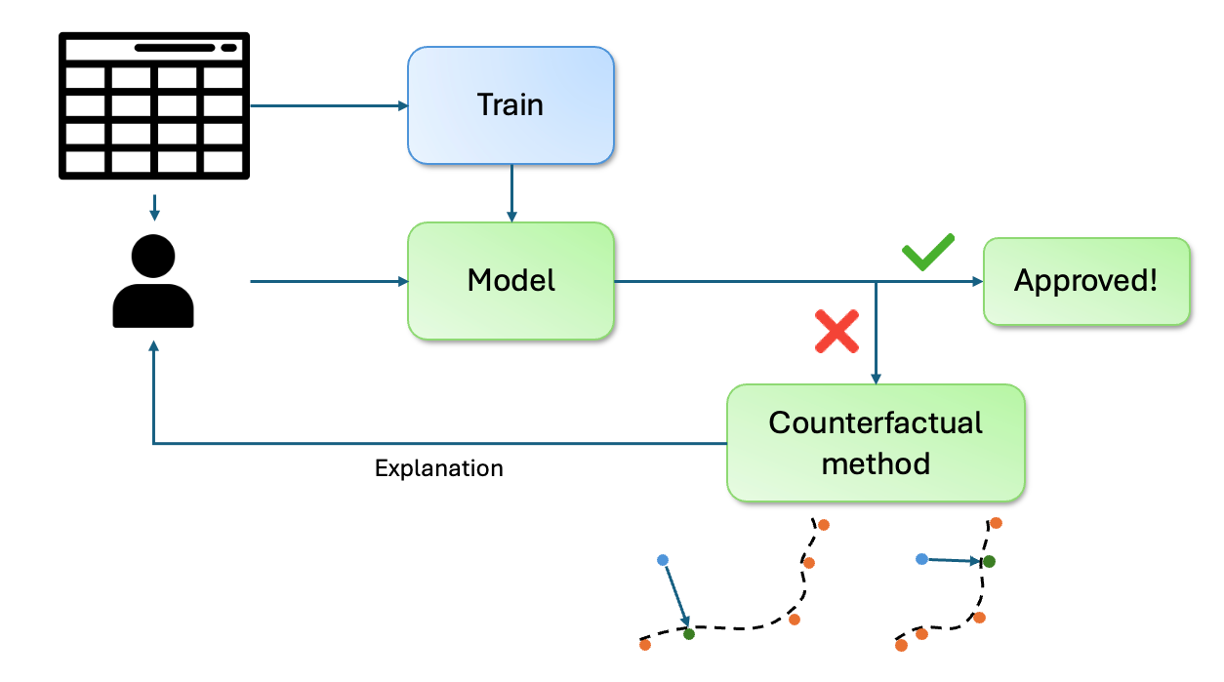
\includegraphics[width=0.4\textwidth]{images/diagram}
\caption{Arquitectura del modelo contrafactual}
\label{fig:architecture_esp}
\end{figure}

\section*{Trabajos Relacionados}
El campo de las explicaciones contrafactuales existe desde hace tiempo y se han propuesto muchos métodos para abordar el problema de explicar redes neuronales. No todos los métodos poseen las mismas propiedades y, a menudo, resulta difícil elegir el más adecuado para un caso de uso concreto. Para ello, \cite{guidotti2024counterfactual} propone un conjunto de propiedades que una buena explicación contrafactual debería cumplir, tales como \emph{validez, minimalidad, similitud, plausibilidad, accionabilidad, diversidad, eficiencia} y \emph{estabilidad}. Algunos métodos como WACH~\cite{wachter2017counterfactual}, ACTREC~\cite{ustun2019actionable}, DiCE~\cite{dice} y SGNCE~\cite{sgnce} se han propuesto para abordar el problema de las explicaciones contrafactuales, pero no satisfacen todas las propiedades mencionadas.

En este proyecto proponemos un método innovador basado en optimización matemática que emplea derivadas de segundo orden para hallar la solución óptima al problema, asegurando la mayoría de las propiedades y estableciendo un marco para trabajos futuros, donde el método pueda mejorarse para cumplirlas todas.

\section*{Metodología}
El método que proponemos formula la generación de contrafactuales mediante multiplicadores de Lagrange. Dada una instancia $\mathbf{x} \in \mathbb{R}^m$, un clasificador diferenciable $M$ y un umbral de decisión $\varepsilon$, buscamos resolver el problema de optimización definido como
\begin{equation}
\label{eq:lagrangian_eqn_es}
\mathcal{L}(\mathbf{x}, \lambda) = C(\mathbf{x}) + \lambda \cdot \Bigl(M(\mathbf{x}) - \varepsilon \Bigr)
\end{equation}

donde $C$ es un función de distancia $\ell_2$ ponderada $C(\mathbf{x}) = \sum_{i=1}^m w_i\bigl(x_i - x_{0,i}\bigr)^2$. Los pesos, modificables por la entidad o el usuario final, codifican el esfuerzo relativo, o coste, de cambiar cada característica $x_i$ respecto a su valor original. Un peso alto significa que cambiar esa característica es difícil o costoso, mientras que un peso bajo indica que es fácil o barato. Esta es la parte clave del método, ya que permite flexibilidad, personalización y accionabilidad.

Para resolver la ecuación \ref{eq:lagrangian_eqn_es}, debemos encontrar el mínimo de la función Lagrangiana $\mathcal{L}$, es decir, hallar los valores que satisfacen $\nabla \mathcal{L}(\mathbf{x}, \lambda) = 0$, donde el sistema de ecuaciones viene dado por

\[
F(\mathbf{x}, \lambda) \;=\; \nabla \mathcal{L}(\mathbf{x}, \lambda) \;=\; 0:\;
\begin{cases}
\nabla C(\mathbf{x}) \; -\; \lambda \cdot \bigl(\nabla M(\mathbf{x})\bigr) \;=\; 0 \\
-\,M(\mathbf{x})\;+\;\varepsilon\;=\;0
\end{cases}
\]

Esto se resuelve mediante una iteración pseudo‑Newton que aprovecha las derivadas de segundo orden para hallar las raíces de $F$. El paso de actualización habitual es

\[
\bigl(\mathbf{x}_{n+1},\,\lambda_{n+1}\bigr)
\;=\;
\bigl(\mathbf{x}_n,\,\lambda_n\bigr)
\; -\;
\mathbf{H}^{-1}\!\bigl(\mathcal{L}(\mathbf{x}_n,\lambda_n)\bigr)
\;\cdot\;
\nabla\mathcal{L}\bigl(\mathbf{x}_n,\lambda_n\bigr).
\]

Como utilizamos la inversa de la matriz Hessiana, las Hessianas mal condicionadas o no invertibles hacen inestable el proceso de optimización. Para mitigar esto, implementamos un paso de actualización alternativo que emplea el gradiente normalizado de la salida del modelo respecto a las características de entrada para actualizar incluso cuando la Hessiana está mal condicionada:

\[
\mathbf{x}_{n+1} = \mathbf{x}_n - \frac{\nabla M(\mathbf{x_n})}{|\nabla M(\mathbf{x_n})|};\;\;
    \lambda_{n+1} = \lambda_n
\]

\subsection*{Tratamiento de características discretas}
Las ecuaciones anteriores suponen que todas las variables de entrada son continuas. Sin embargo, en los conjuntos de datos reales no todas las variables son numéricas. Por ejemplo, si se utiliza el número de líneas de crédito como variable de entrada, esta no puede tomar un valor decimal. Se necesita un regularizador adaptativo que obligue a la variable de entrada a colapsar a un valor entero:

\[
R(\mathbf{x})=\sum_{i:\, x_i\in \mathcal{Z}}\bigl(x_i-\lfloor x_i\rceil\bigr)^2
\]

Este regularizador se introduce en $C$ sólo cuando la iteración está cerca de la solución óptima, forzando las características enteras hacia valores enteros. Las características categóricas se codifican en one‑hot, pero aún no hemos implementado un modo de manejarlas en el método.

\section*{Evaluación Empírica}
Para evaluar, utilizamos diferentes conjuntos de datos~\cite{kaggleLoan1,spambase,santander} que van desde 8 hasta 200 características. Las métricas que evaluamos son: validez, similitud, plausibilidad, eficiencia, estabilidad y accionabilidad.
\begin{enumerate}
\item \textbf{Validez y Similitud.} El algoritmo de Newton encuentra el cambio mínimo necesario para alterar la salida de clasificación del modelo para una muestra específica.
\item \textbf{Plausibilidad.} El 100\% de las explicaciones generadas se encuentran dentro de los límites del conjunto de datos original y no eran \emph{outliers}.
\item \textbf{Eficiencia.} Tiempos de ejecución entre $0.02$ y $0.16$ segundos en los conjuntos utilizados, aproximadamente $10\times$ más rápido que DiCE~\cite{dice} y más de $100\times$ más rápido que SGNCE~\cite{sgnce}.
\item \textbf{Estabilidad.} Ratios de distancia contrafactuales $\approx0.8$–$1.0$, mostrando resultados estables.
\item \textbf{Accionabilidad.} Permitimos al usuario definir los pesos, codificando la dificultad de cambiar cada característica, lo que posibilita contrafactuales diversos y realistas.
\end{enumerate}

\section*{Aplicación Web}
Se ha desarrollado un sitio web en \texttt{streamlit} que muestra las capacidades del modelo, permitiendo a los usuarios generar contrafactuales de forma interactiva. Es una interfaz personalizable que funciona con cualquier conjunto de datos y consiste en un formulario donde el cliente introduce sus datos personales y el conjunto de pesos que desea utilizar. Si el modelo produce una clasificación negativa para los datos introducidos, el metodo generará el contrafactual y mostrará al usuario los cambios necesarios para invertir la decisión. El código para reproducir esta web está disponible en: \url{https://github.com/javiprietod/TFG}

\section*{Conclusiones y Trabajo Futuro}
Este trabajo presenta el primer algoritmo de explicaciones contrafactuales cuyo procedimiento de búsqueda se basa íntegramente en optimización de Newton. Un vector de pesos dentro de la función de coste codifica la dificultad real de modificar cada característica, de modo que los analistas o usuarios finales pueden declarar ciertos atributos como inmutables (p. ej. la edad) o hacer otros baratos de cambiar. Esta novedosa codificación de la realidad no se ha encontrado aún en ningún método de la literatura.

El trabajo futuro contempla cuatro extensiones: (1) añadir un regularizador para minimizar el \emph{número} de características modificadas, equilibrando similitud frente a minimalidad; (2) aprender un vector de pesos inicial informado a partir del feedback histórico de los usuarios para que el sistema parta de costes que previamente hayan generado contrafactuales más accionables; (3) ampliar el método para trabajar con características categóricas codificadas en one‑hot; y (4) colaborar con agentes del sector para desplegar nuestra solución en escenarios reales. Conjuntamente, estas líneas pretenden personalizar aún más las explicaciones y ampliar la compatibilidad con distintos conjuntos de datos.

\newpage
\setcounter{page}{1}
\fancyfoot[C]{
    \begin{center}
        \thepage
    \end{center}
} 
\renewcommand{\footrulewidth}{0.4pt}
\setlength{\footskip}{0.8cm}
%%%%%%%%%%%%%%%%%%%%%%%%%%%%%%%%%%%%%%%%%%%%%%%%%%%%%%%%
%%%% Introduction %%%%%%%%%%%%%%%%%%%%%%%%%%%%%%%%%%%%%%
%%%%%%%%%%%%%%%%%%%%%%%%%%%%%%%%%%%%%%%%%%%%%%%%%%%%%%%%
\section{Introduction}
Currently, the regulations many entities face on the use of AI are very restrictive. They must be able to ``explain" the decisions made by their models to justify business decisions based on those AI systems~\cite{cohen2021black}. Today, the vast majority of them use models such as decision trees, random forests, and logistic regressions due to the lack of interpretability of more powerful models~\cite{ghatasheh2014business,pointofview}. 

The aim of this project is to provide a solution for two main problems. First, neural networks and larger models are considered ``black-box" models, so we cannot fully understand the decision-making processes behind specific outputs, and therefore result useless when facing regulations. Secondly, we wish to give \emph{actionable} solutions for differentiable classification models, such as neural networks or logistic regressions, by identifying changes in input features that could alter the model output. In the context of banking and loan applications, for example, if a loan application is denied, the solution should provide actionable insights, such as ``reduce your debt by \$10,000 to qualify" or ``increase your salary by \$5,000 to qualify." These are concrete changes in the individual's profile that can change the classification outcome. These \emph{explanations} or actionable changes are known as \emph{counterfactuals}~\cite{wachter2017counterfactual,guidotti2024counterfactual}. A counterfactual reveals what should have been different in an instance to observe a different outcome. These explanations are a clear and direct definition for local interpretability. It provides an insight into why a singular instance has been classified a certain way. For our specific case, our aim is not to solve or provide global interpretability, as the end user, or clients of a bank, do not need to know the reason a model behaves a certain way for the entire dataset.

Our objective is to devise a novel counterfactual technique based on an \emph{optimal mathematical solution} to the problem, using optimization methods and the model's derivatives to find the minimal shift needed for a given instance to change its output. We propose a innovative solution in which the end user is able to weigh how easy or difficult is to change each of the original features.

In Section \ref{sec:related} we discuss related works in the field of counterfactual explanations, highlighting the properties a good explanation should fulfill and the current state-of-the-art methods. In Section \ref{sec:methodology} presents the methodology used in this project, including the mathematical formulation of the problem (Subsections \ref{sec:mathematical} and \ref{sec:singular}), the use of weights to shape the distance function (Subsection \ref{sec:weights}), the handling of actionability (Subsections \ref{sec:discrete} and \ref{sec:enforcing_plausibility}), and the implementation details(\autoref{alg:newton_counterfactual} and Subsections \ref{sec:threshold} and \ref{sec:stopping}). We evaluate the proposed method in Section \ref{sec:evaluation}, where we analyse each of the properties we fulfill in depth and we show the website created in Section \ref{sec:website}
Finally, we conclude the project in Section \ref{sec:conclusion} and discuss future work. The code is available at \url{https://github.com/javiprietod/TFG}

%%%%%%%%%%%%%%%%%%%%%%%%%%%%%%%%%%%%%%%%%%%%%%%%%%%%%%%%
%%%% Related works %%%%%%%%%%%%%%%%%%%%%%%%%%%%%%%%%%%%%
%%%%%%%%%%%%%%%%%%%%%%%%%%%%%%%%%%%%%%%%%%%%%%%%%%%%%%%%
\section{Related work}\label{sec:related} 
Research in counterfactual explanations often highlights a set of properties a good explanation should fulfill~\cite{guidotti2024counterfactual}. These are:
\begin{itemize}
  \item \textbf{Validity:} The counterfactual truly changes the classification outcome.
  \item \textbf{Minimality:} The counterfactual changes only the smallest necessary set of features.
  \item \textbf{Similarity:} The counterfactual remains close to the original instance by some distance metric.
  \item \textbf{Plausibility:} The counterfactual resembles realistic feature values found in the reference dataset.
  \item \textbf{Actionability:} The counterfactual only changes features that can realistically be altered (e.g., debt reduction might change but not the applicant's age).
  \item \textbf{Diversity:} A set of counterfactuals should offer varied options for achieving the desired outcome.
\end{itemize}

Other desirable properties of the explanation \emph{itself} are efficiency, related to the computational resources needed to obtain the explanations; stability, if two instances are similar, their counterfactual explanations should be similar as well; and fairness, explanation remains valid even if sensitive attributes (e.g., ethnicity) were altered~\cite{guidotti2024counterfactual}.

Counterfactual methods can be categorized by the strategy used to create the explanations. The main strategies include Optimization-based, Heuristic-based, Instance-based, and Decision-tree-based methods~\cite{guidotti2024counterfactual}. While optimization-based explainers usually have outstanding results in many of the individual properties highlighted above, they usually lack a good trade-off between all of them. Heuristic, instance and decision tree based methods are usually endogenous, meaning the counterfactual returned comes from the original dataset, which provides good results for plausibility and diversity, but not for similarity. On the other hand, optimization methods are in their majority exogenous, meaning they create a new sample based on the algorithm they follow, which usually performs good on minimality and similarity while possibly leaving other properties like plausibility and actionability unfulfilled. The current state-of-the-art does not yet include an explainer that fulfills all the desirable properties~\cite{guidotti2024counterfactual}.

The task of finding an algorithm that fulfills all of the properties has been attempted in many papers. The most well-known technique in counterfactual space is WACH~\cite{wachter2017counterfactual}, one of the first papers to publish and propose these explanations. They propose a loss function, adopted by other explainers, consisting in a distance function and a cross-entropy loss, which they try to minimize with a common optimizer such as SGD~\cite{sgd} or Adam~\cite{adam}. While it is a good starting point, it does not guarantee the optimal solution, and it is not guaranteed to converge to a solution that fulfills all the properties mentioned above.

Among the more rigorous contributions, ACTREC (Actionable Recourse)~\cite{ustun2019actionable}, is one of the first to address which features can be changed and which must remain fixed. ACTREC formulates the counterfactual generation as a discrete optimization problem using integer programming, ensuring feasibility, actionability, and minimal cost over a discretized space. It guarantees global optimality within its constraints but is limited to linear models and can become computationally intensive for high-dimensional problems

Another notable method is DiCE~\cite{dice}, which uses a differentiable loss function to generate a set of diverse counterfactuals. DiCE ensures validity and similarity while promoting diversity using Determinantal Point Processes~\cite{dpprocess}. While many methods focus on finding the closest counterfactual with high precision, DiCE offers users a broad range of actionable options not ensuring the closest counterfactual. 

Finally, SGNCE (Scaling Guarantees for Nearest Counterfactual Explanations)~\cite{sgnce} guarantees the closest actionable counterfactual by formulating the search as a mixed-integer programming (MIP) problem, exploring the full solution space and supporting variables of mixed types. This approach provides formal guarantees on coverage, feasibility and similarity, making it robust but computationally demanding. Unlike SGNCE, our method achieves similar goals through a continuous, second-order optimization strategy that avoids combinatorial search. By doing so, we gain significant efficiency and maintain similarity, while still enabling tailored cost functions and domain-specific adaptations; an advantage in real-world sectors like finance.

Other common XAI methods like LIME~\cite{lime} and SHAP~\cite{shap} exist, but they provide explanations by assigning feature importance rather than producing clear, actionable changes in the input that could alter the classification. They both have adapted to the counterfactual world~\cite{limecshapc} but are mainly adapted to textual data and it has not been compared with many of the algorithms in the literature~\cite{guidotti2024counterfactual}.

Our objective is to devise a novel counterfactual technique based on the \emph{optimal mathematical solution} to the problem, using optimization methods and the model's derivatives to find the minimal shift needed for a given instance to change its output, fitting into the optimization-based category. We not only fulfill this similarity to the original instance by minimizing a distance function, validity and plausibility are guaranteed as well with the intrinsics of the method. Other features like minimality (of features changed), actionability, and diversity are achieved through a set of weights that impact the decisions and inner workings of the method in every step. This gives the ability, to either the entity that provides the service or the end-user, to determine which features are actually changeable and how difficult it is to change each of them. For example, in a certain situation, the user might feel more comfortable increasing their salary than reducing the loan amount. As these weights can be changed, our method has the ability to provide a wide spectrum of explanations, adapting to every situation and the needs and interests of different parties.

%%%%%%%%%%%%%%%%%%%%%%%%%%%%%%%%%%%%%%%%%%%%%%%%%%%%%%%%
%%%% Methodology %%%%%%%%%%%%%%%%%%%%%%%%%%%%%%%%%%%%%%%
%%%%%%%%%%%%%%%%%%%%%%%%%%%%%%%%%%%%%%%%%%%%%%%%%%%%%%%%
\section{Methodology}\label{sec:methodology}
The purpose of this project is to create a innovative XAI technique for differentiable models. We will initially restrict the analysis to differentiable models since the method requires the use of derivatives for optimization matters and for that, differentiability is needed. We will also assume that it is a binary classification model with a threshold to determine the change in the target variable. This new technique, or method, falls into the Counterfactual Explanations family of XAI. As mentioned earlier in the motivation, a counterfactual reveals what should have been different in an instance to observe a diverse outcome.

Following the definition of a counterfactual, and inspired by some of the main properties mentioned earlier, the innovative method aims to fulfill as many properties as possible. With the validity and similarity properties in mind, which refer to counterfactuals that succeed in changing the classification output with the minimum change needed, the mathematical optimization method of Lagrange multipliers~\cite{lagrange} comes up with a direct application to the problem. In this optimization method, it is possible to find local minimum (or maximum but it does not apply to the problem) of a function with certain equation constraints. In the case of the counterfactual, we want to find a point that minimizes the distance with respect to the original instance, subject to the condition of changing its classification output. This would fulfill both of the properties mentioned above. The equation with the Lagrangian multiplier becomes
\begin{equation}\label{eq:lagrange}
\mathcal{L}(\mathbf{x}, \lambda) = \; C(\mathbf{x}) + \lambda \, \Bigl(M(\mathbf{x}) - \theta \Bigr),
\end{equation}
where
\begin{itemize}
  \item $x$ is the new instance (the counterfactual) with m features,
  \item $C(\cdot)$ is a weighted cost function (distance) measuring how far $x$ is from its original instance,
  \item $M(\cdot)$ is a differentiable model, 
  \item $\theta$ is the threshold for changing the classification,
  \item $\lambda$ is the Lagrange multiplier.
\end{itemize}
The base of the cost/distance function is the weighted $L^2$ norm, which can be defined as follows.
\begin{equation}\label{eq:cost}
    C(\mathbf{x}) = \sum_{i=1}^{m} \mathbf{w}_i \cdot (\mathbf{x}_i - \mathbf{x}^0_{i})^2,
\end{equation}
where $x^0$ is the original instance and $w$ is the weight vector.

We will discuss added regularizers added to this cost function later, but the main idea is to have a distance function that can be weighted by the user, or the entity using the method, to determine how easy or difficult it is to change each feature. This is a key part of the method, as it allows for flexibility and customization in the counterfactual generation process.

\subsection{Mathematical solution}\label{sec:mathematical}
The minimum value of $\mathcal{L}$ is found when the partial derivatives 
w.r.t.\ $\mathbf{x}$ and $\lambda$ are equal to 0. This implies:
\begin{equation}\label{eq:deriv}
F(\mathbf{x}, \lambda) \;=\; \nabla \mathcal{L}(\mathbf{x}, \lambda) \;=\; 0:
\begin{cases}
\nabla C(\mathbf{x}) \;-\;\lambda \cdot \bigl(\nabla M(\mathbf{x})\bigr) \;=\; 0 \\
-\,M(\mathbf{x})\;+\;\varepsilon\;=\;0
\end{cases}
\end{equation}
To solve this problem we will use the \emph{Newton-Raphson} method to solve this mathematical problem, ensuring we reach the optimal solution. Newton's method is used to find the roots of a function, or the solution to the equation $f(x) = 0$. In optimization, with $f \in C^2$, we are trying to find the roots of $f'$, or the solutions to $f'(x) = 0$, known as critical points. These points can be minima, maxima or saddle points, but in the case of this problem we will try to find the minima of the function $f$. \par
For this, Newton-Raphson’s method of optimization uses the first and second term of the Taylor expansion of the function to find that point iteratively~\cite{fliege2009newton}. For 1 dimension, or 1 variable, the update rule is $x_{k+1}=x_{k}-{\frac {f'(x_{k})}{f''(x_{k})}}$. As seen in \eqref{eq:deriv}, we have at least two variables ($x$ and $\lambda$), so the we have to use the generalization of the iterative scheme using the hessian as the second derivative. Thus, the new iterative scheme obtained becomes
\begin{equation}\label{eq:newton}
\bigl(\mathbf{x}_{n+1},\,\lambda_{n+1}\bigr)
\;=\;
\bigl(\mathbf{x}_n,\,\lambda_n\bigr)
\;-\;
\mathbf{H}^{-1}\!\bigl(\mathcal{L}(\mathbf{x}_n,\lambda_n)\bigr)
\;\cdot\;
\nabla\mathcal{L}\bigl(\mathbf{x}_n,\lambda_n\bigr).
\end{equation}
If we set $F(\mathbf{x},\lambda) \;=\;\nabla \mathcal{L}(\mathbf{x},\lambda)$, 
the equation simplifies to
\begin{equation}\label{eq:newton_simplified}
\bigl(\mathbf{x}_{n+1},\,\lambda_{n+1}\bigr)
\;=\;
\bigl(\mathbf{x}_n,\,\lambda_n\bigr)
\;-\;
\mathbf{J}\!\bigl(F(\mathbf{x}_n,\lambda_n)\bigr)
\;\cdot\;
F\!\bigl(\mathbf{x}_n,\lambda_n\bigr),
\end{equation}
where
\begin{equation}\label{eq:hessian}
\mathbf{J}\!\bigl(F(\mathbf{x}_n,\lambda_n)\bigr)
\;=\;
\begin{pmatrix}
H\!\bigl(C(\mathbf{x}_n)\bigr)\;-\;\lambda_n \cdot H\!\bigl(M(\mathbf{x}_n)\bigr) 
    & -\,\nabla M(\mathbf{x}_n)
\\[6pt]
-\,\nabla M(\mathbf{x}_n)
    & 0
\end{pmatrix}.
\end{equation}
Above, $H(\cdot)$ denotes the Hessian (second derivative) with respect to $\mathbf{x}$, 
and $\nabla(\cdot)$ denotes the gradient (first derivative)

A similar method of optimizing a loss function has been done in the past (BFGS \cite{papakonstantinou2009historical}), 
but due to the computational complexity of calculating second derivatives, most of the work has been with its approximations. In this case, we will employ \emph{autograd}, PyTorch's automatic differentiation engine to calculate these second derivatives efficiently, eliminating the need for approximations. User must take into account that this method can only be applied with at least twice-differentiable models.

Although optimal, this mathematical approach has some challenges. First, in some iterations of some datapoints, the hessian can become singular or ill-conditioned, making the update step unfeasible to compute. This causes problems to the overall convergence of the method for that certain point. 
Second, many real-life datasets include variables like integer and categorical columns. The method works very well with continuous variables but it does not have a direct and easy solution for dealing with these column types.

\subsection{Singular matrices}\label{sec:singular}
As discussed, one of the main problems when taking this optimization-based generation is the possibility of singular or ill-conditioned Hessians. This can most tipically happen because of two main causes. If we have two variables that have a high correlation, the hessian  will most likely have a very small eigenvalue associated, which means that the matrix could become ill-conditioned or even singular. This is very easily solved by performing a bit of exploratory data analysis and removing highly correlated variables. This is already a common practice in the field, so it is assumed that it should not produce any problems.

The second problem is harder to solve, and it is the one we will be discussing in this section. This problem appears when the gradient of the model is very close to 0, or the model has a flat curvature around a particular input. This leads again to a small eigenvalue, and the matrix becomes ill-conditioned. Common approaches to solve this problem, such as pseudo-inverse, damping techniques or using first-order updates, were applied unsuccesfully. Therefore, in order to mitigate this issue, we implement an alternative update strategy when the gradient of the model is below a certain threshold. %this type of ill-conditioning in the Hessian is detected (\textcolor{red}{How is detected?}).

The alternative update step devised consists of using the normalized gradient of the model's output with respect to the input features to update. 
\begin{equation}
    \begin{cases}
    \mathbf{x}_{n+1} = \mathbf{x}_n - \frac{\nabla M(\mathbf{x_n})}{|\nabla M(\mathbf{x_n})|}
    \\
    \lambda_{n+1} = \lambda_n
    \end{cases}
\end{equation}

This update step is designed to move the input in the direction of the gradient of the model's output with respect to the input features, but more importantly, it works as a nudge in a direction to exit the flat region of the model. This update step proved very effective in practice, as it allows the algorithm to continue making progress towards a valid counterfactual even when the Hessian is ill-conditioned. 

\subsection{How weights shape the distance}\label{sec:weights}
In our counterfactual explanation framework, the distance function~\eqref{eq:cost} quantifies how “far” a candidate counterfactual \(\mathbf{x}'\) lies from the original instance \(\mathbf{x}\), where \(w_i \ge 0\) encodes the relative “cost” or difficulty of changing feature \(i\).

\begin{itemize}
  \item \textbf{High weights} (\(w_i \!\!\gg\! 1\)) make changes in feature \(i\) “expensive”, discouraging the optimization from selecting that feature unless it is indispensable for flipping the model output.
  \item \textbf{Low weights} (\(w_i \!\!\approx\! 0\)) make changes in feature \(i\) “cheap”, biasing counterfactuals toward modifying \(x_i\) first.
\end{itemize}
By tuning the vector \(\mathbf{w}\), practitioners can encode domain knowledge about which features are easy or hard to change in the real world, and users can tune their explanations by encoding their desirability or actionability to alter some features over others.

In practice, one might begin with all $w_i = 1$ (equal cost), inspect the resulting explanation, and then increase $w_i$ for features the end user finds unrealistic or non‐actionable, thereby refining the counterfactuals to be truly \emph{actionable}. We will analyse actionability in Section \ref{sec:actionability}.

\subsection{Discrete features}\label{sec:discrete}
To address discrete variables, we impose a regularizer to the distance function worked the best for the task. The regularizer is designed to have minima at the integer points, so Newton's method converges to one of those points.

% {\color{red} Resumir! Quita todo lo que no sea el regularizador definitivo


% We explored different trigonometric funcions, such as sines and cosines with periods matching the integers, but some features were getting stuck on the maxima of that function, as it has derivative 0 as well and Newton's method is designed to find critical points in general. One of the functions proposed for solving the discrete challenge faced was
% \begin{equation}
%     tan(\pi * x)^2
% \end{equation}
% that looks like
% \begin{figure}[H]
%     \centering
%     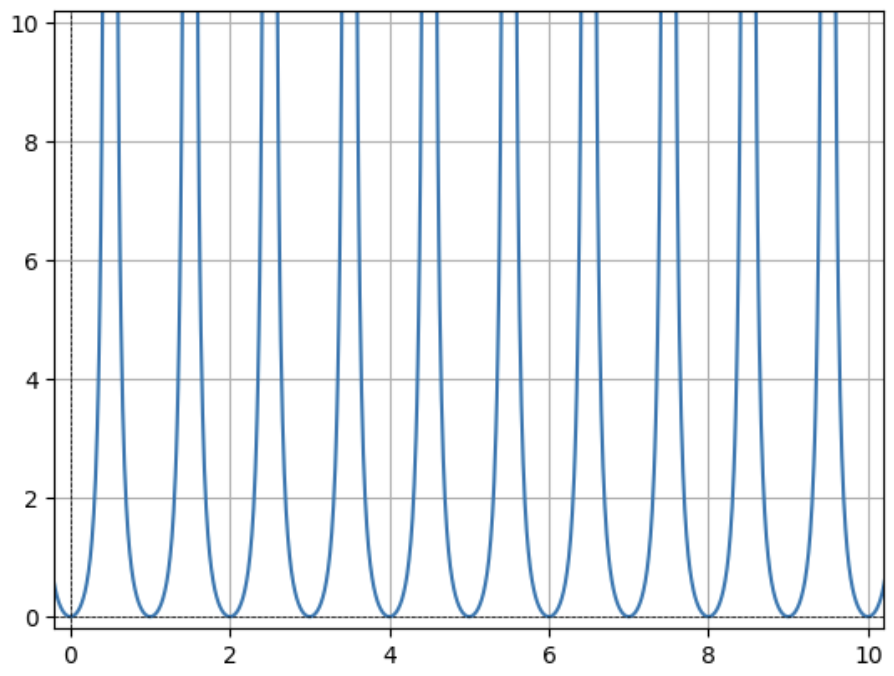
\includegraphics[width=0.5\textwidth]{images/tan_integers}
%     \caption{Tangent regularizer function}
%     \label{fig:reg tan}
% \end{figure}
% This function takes the value 0 in the integer points, but more importantly, they are minima, which are critical points in the newton's method. This means that iteratively, the features where the regularization is enforced will end up in one of those points because the Newton's method aims to find the points that make $f'(x) = 0$. This function works well in practice and with the newton method, but we proposed a better solution that works even better in practice. 
The function proposed for this regularizer is
\begin{equation}
    (x - \left\lfloor x \right\rceil )^2
\end{equation}
that looks like
\begin{figure}[H]
    \centering
    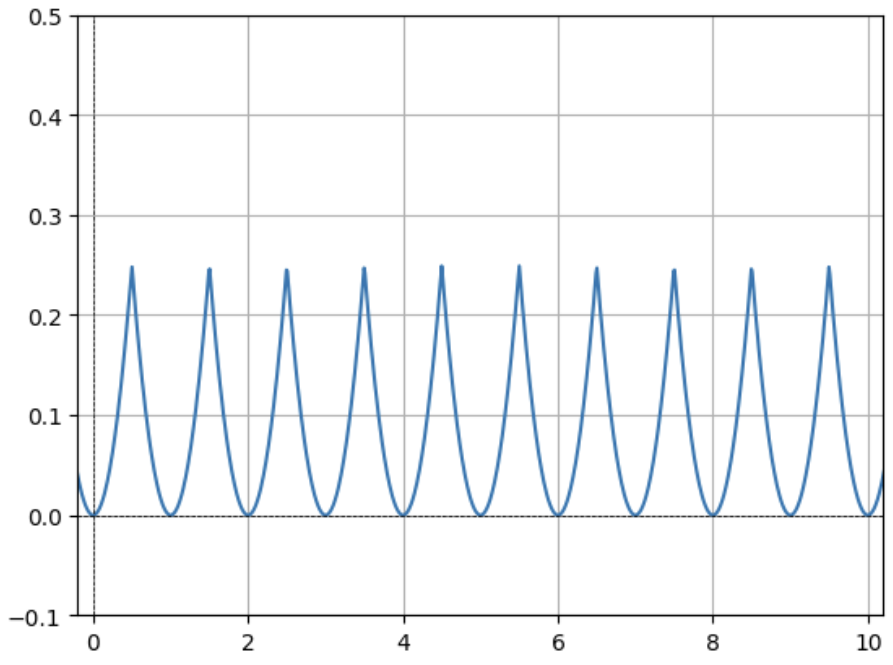
\includegraphics[width=0.5\textwidth]{images/round_integers}
    \caption{Round regularizer function that has null derivative in the integer values in the X axis}
    \label{fig:reg round}
\end{figure}
% We say it works better beacause it reaches the same solution as the tangent function, but it is much more stable, faster and easier to compute. As the tangent funcion takes the value $\infty$ in the values exactly between integers, the gradients it takes are very big and the updates are very big as well, which leads to more inestability. The round function, on the other hand, takes the value 0 in the integers and 0.25 as its maximum, so it is much more stable and easier to compute. In theory, any function whose derivative is only 0 in the integers should work.

% This regularizer is added to the cost function, so the new cost function becomes
% \begin{equation}\label{eq:cost_reg_unscaled}
%     C(\mathbf{x}, \mathbf{x}', \mathbf{w}) = \sum_{i=1}^{m} \mathbf{w}_i \cdot (\mathbf{x}_i - \mathbf{x}'_{i})^2 + \sum_{i=1}^{m} (x - \left\lfloor x \right\rceil )^2 \cdot \mathbf{1}_{\{x_{i}\in\mathbb{Z}\}}
% \end{equation}
% }

A common practice in data-science is to standardize the data, meaning that the features are transformed to have mean 0 and standard deviation 1, helping the model to converge faster and better. If the features are standardized, the regularizer will not work as expected. In this case, we can use a scaled version of the regularizer, which is designed to work with standardized features. The scaled version of the regularizer is defined as
\begin{equation}\label{eq:cost_reg_scaled}
    C(\mathbf{x}, \mathbf{x}', \mathbf{w}) = \sum_{i=1}^{m} \mathbf{w}_i \cdot (\mathbf{x}_i - \mathbf{x}'_{i})^2 + \sum_{i:\, x_i\in \mathcal{Z}} (x_i \cdot std_i + mean_i - \left\lfloor x_i \cdot std_i + mean_i \right\rceil )^2
\end{equation}
where \(std_i\) and \(mean_i\) are the standard deviation and mean of the \(i^{th}\) feature respectively, previously calculated with the whole dataset before training the model. 

Nevertheless, we will not use this regularizer in every iteration. This regularizer is not designed to find the optimal solution with the integer features, it is designed to find \emph{any} integer solution. For that, we want to approach the optimal solution first without taking into account the integer features, so that the solution with integers comes close to the optimal solution. Then, we incude the regularizer in the cost function, so the algorithm converges to the closest solution in which the integer columns are very close to being integers. When it is reaching the optimal solution with the regularizer, we disable the regularizer, round the features to the closest integer and disable them by setting the weights to $\infty$, so that it is virtually impossible to change that feature. After that, we continue the optimization process with the variables left to reach the optimal solution with the integer features frozen. A detailed algorithm of the process is shown in \autoref{alg:newton_counterfactual}.

\textcolor{red}{Estaria bien una imagen que ilustre como funcione este proceso}

\subsection{Enforcing plausibility}\label{sec:enforcing_plausibility}
Another important property of counterfactuals is plausibility, which refers to the fact that the counterfactual should be a realistic and feasible instance. In our case, we want to ensure that the counterfactuals generated are plausible in the context of the problem at hand. To achieve this, we can use a set of constraints that limit the range of values that the features can take. These constraints can be defined based on domain knowledge, expert opinion or the data distribution in general. For example, if we are working with a dataset of bank customers, we can set constraints on the range of values that the features can take, such as the minimum and maximum values for each feature. This way, we can ensure that the counterfactuals generated are plausible and realistic in the context of the problem at hand

In practice, we can implement these constraints by clamping the values of the features to their respective ranges, as we are lacking expert knowledge. This means that if a feature value goes below its minimum or above its maximum, it will be set to the closest valid value. 

\subsection{Single variable optimization}\label{sec:single}
As mentioned in the previous sections, features can be deactivated from the optimization process and frozen in value for reasons such as integer regularization or plausibility. Lagrange multipliers are a common way to optimize a multivariate function with restrictions. In the case of one variable, the problem becomes one-dimensional and it is easy to find the roots of the function $M(x) = \varepsilon$ using Newton's root finding method:
\begin{equation}
    x_{n+1} = x_n - \frac{M(x_n) - \varepsilon}{\nabla M(x_n)}.
\end{equation}
Note that this process cannot be carried out with two or more variables, as $\nabla C(x)$ and $\nabla M(x)$ are vectors and therefore the solution to $\mathcal{L}(x, \lambda) = 0$ is not as trivial as a root finding algorithm.

\subsection{Threshold}\label{sec:threshold}
The threshold is a key part of the method. For starters, it is the value that determines whether the model output changes or not. The threshold can be set to any value, but is usually set to 0.5 for binary classification problems. Abstracting ourselves from the mathematical problem and counterfactual generations, we want this to be useful in a real-world scenario. 

It is a common practice for companies to update their models by retraining them with more data to make them more robust. As the counterfactual method is designed to find the minimal change given that the model's output is equal to the threshold, if we match that threshold to the \emph{business decision threshold} (the one the banks use to finally determine whether to give out a loan or not), it creates a risk of the counterfactuals not being useful in the future because of those model updates. For this reason, we can set the optimization objective to $0.5 + \varepsilon$, making the model believe that the counterfactual is more likely to be approved. This ensures that the counterfactuals generated will be valid and useful in the future.
% \textcolor{red}{No entiendo esta frase siguiente} For this reason, we can set the threshold to be $0.5 + 10^{-5}$ or $0.5 + 10^{-7}$, which is a small value that ensures that the counterfactuals generated will be valid and useful in the future.


%\textcolor{red}{Reescribir: Another reason to set the threshold to the business decision threshold + a small value is due to two little errors that can appear.} 
Newton's method is known to have a convergence problem for some functions, getting stuck in a \emph{2-cycle}, never reaching the optimal solution~\cite{ypmanewton}. These cycles can happen anytime in the optimization process, and they can be of any length. During the algorithm testing phase, we have not encountered any \emph{2-cycle} larger than $10^{-8}$.

In addition to these cycles appearing, floating-point can appear as well. In some of our experiments using $0.5$ as a threshold, even if Newton's algorithm converged to a solution without any cycles appearing, the counterfactual failed the validity check due to small rounding errors.

For all of these reasons, we set the threshold to $0.5 + 10^{-5}$ or $0.5 + 10^{-7}$ (with $\varepsilon$ taking a value larger than $10^{-8}$), maintaining similarity to the original instance and ensuring validity in the counterfactual generated. 

%\textcolor{red}{Reescribir: Another reason to set the threshold to a value bigger than $0.5$ is due to floating-point errors. When working with floating-point numbers, it is common to encounter small errors due to the way numbers are represented in computers. When setting the threshold to $0.5$, we encountered some problems when checking the validity of the counterfactual, and even though the method converged to a solution, the counterfactual was not valid because of these errors. This is yet another reason to set the threshold to a value bigger than $0.5$. Other methods in the literature have also set the threshold to a value bigger than $0.5$~\cite{sgnce}, but they have different reasons to do so, like complexity or computational cost. We do not have these problems, as our method converges to the optimal solution for a given threshold, but for the reasons mentioned above, we set the threshold to a value bigger than $0.5$.}

\subsection{Obtaining the counterfactuals}\label{sec:obtaining_counterfactuals}
We can now obtain the counterfactuals by iteratively applying the Newton-Raphson method to the Lagrangian function~\eqref{eq:lagrange} with the cost function~\eqref{eq:cost_reg_scaled}. The algorithm is detailed in \autoref{alg:newton_counterfactual}. This is a general algorithm that can be used on any fully numerical dataset, but it needs some modifications to obtain the results explained in the next section.

When using the alternative update step for ill conditioned Hessians explained in Section \ref{sec:singular}, we have to determine when to use it. As we do not want to be influenced by the number of features, we use the infinity norm of the model's derivative with respect to the input features (line \ref{lst:line_norm}), which corresponds as well with the jacobian of the model with respect to lambda (see \eqref{eq:hessian}). When this norm is below a certain threshold, we consider the Hessian to be ill-conditioned and we use the alternative update step. As we are using the model's derivative, it is model dependent, and therefore, it is dataset dependent as well. We have used values between $0.05$ and $0.2$ for the threshold, but it is a value that can be set by the entity using the method. The lower the value, the more often the alternative update step will be used, which can lead to a slower convergence, but it is a trade-off that can not always be made due to the models derivative.

\begin{algorithm}
    \caption{Newton's Method for Counterfactual Explanations}
\label{alg:newton_counterfactual}
\begin{algorithmic}[1]
    \Function {$\textsc{newton\_optimization}(\mathbf{p},M, w)$} {} 
    \State $\mathbf{p}_{\text{new}} \gets \mathbf{p}$
    ,\; $\lambda \sim N(0, 1)$
    ,\;$\mathbf{continue} \gets true$
    ,\; $first\_time \gets true$
    ,\; $thres\_term \gets \text{threshold} - M(\mathbf{p}_{\text{new}})$
    \While{\textbf{continue} \textbf{and} epochs $<$ max\_epochs}
        \If{$|thres\_term| < 0.1 \land first\_time \land \text{epochs} > 1$} \Comment{close to threshold}
            \State $reg\_int \gets true$
            \State $first\_time \gets False$
        \EndIf
        \State Reset gradients of $\mathbf{p}_{\text{new}}$ and $\lambda$
        \Function{$\textsc{FplFunc}(\mathbf{x},\lambda)$} {}\Comment{first-order derivative of Lagrangian}
            \State $g_{d} \gets \nabla C(\mathbf{x})$
            ,\;$g_{r} \gets \nabla M(\mathbf{x})$
            \State \Return $\bigl[g_{d}-\lambda\,g_{r},\;(\text{threshold}-M(\mathbf{x}))\bigr]$
        \EndFunction
        \State $\mathbf{fpl} \gets \textsc{FplFunc}(\mathbf{p}_{\text{new}},\lambda)$
        \State $J \gets \text{Jacobian}\!\bigl(\textsc{FplFunc},
                            (\mathbf{p}_{\text{new}},\lambda)\bigr)$
        \If{$\Vert J_{\lambda}\Vert_{\infty}<\varepsilon$}\label{lst:line_norm} \Comment{ill-conditioned}
            \State $\delta \gets thres\_term\ \cdot
                    \Bigl[\frac{\nabla M(\mathbf{p}_{\text{new}})}{|\nabla M(\mathbf{p}_{\text{new}})|},\;0\Bigr]$
        \Else
            \State $\delta \gets J^{-1} \cdot \mathbf{fpl}$ \Comment{Newton step}
        \EndIf
        \State $\mathbf{p}_{\text{new}}[w_{active}] \gets 
                \mathbf{p}_{\text{new}}[w_{active}]- \delta[w_{active}] $
        \State $\lambda \gets \lambda - \delta_{-1}$
        \If{$|thres\_term|<0.1 \land epochs>1 \land reg\_clamp$}
            \State Clamp $\mathbf{p}_{\text{new}}$ to valid bounds 
            \State Deactivate out-of-bounds feature in $w$
        \EndIf
        \State Evaluate $thres\_term \gets \text{threshold}-M(\mathbf{p}_{\text{new}})$
        \State $epochs \gets epochs+1$
        \State \textbf{continue} $\gets (thres\_term>0)\lor
                \dfrac{\lVert\delta\rVert}{\lVert[\mathbf{p}_{\text{new}},\lambda]\rVert}>\varepsilon$
        \If{\textbf{not} \textbf{continue} \textbf{and} $reg\_int$}
            \State Round integer features;\; disable $reg\_int$;\; deactivate integer features
            \State \textbf{continue}$\gets$true
        \EndIf
    \EndWhile
    \State \Return $\mathbf{p}_{\text{new}}$
    \EndFunction
\end{algorithmic}
\end{algorithm}

\subsection{Stopping criteria}\label{sec:stopping}

The Newton–Raphson loop (\autoref{alg:newton_counterfactual}) terminates when
\emph{all} of the following safeguards are satisfied:\footnote{Classical
discussions of termination for Newton‐type methods can be found in
\cite{numopt}}

\begin{enumerate}
  \item \textbf{Feasibility of the classifier constraint.}  
        We stop only after the current point $\mathbf{p}_{\text{new}}$ has crossed the decision boundary, or equivalently, when the $\textit{threshold}-M(\mathbf{p}_{\text{new}})\le 0$. This criterion guarantees that the produced counterfactual is indeed assigned to the desired target class.
  \item \textbf{Sufficiently small Newton step.}  
        The relative update $\tfrac{\lVert\delta\rVert}{\lVert[\mathbf{p}_{\text{new}},\lambda]\rVert}$ must fall below a tolerance $\delta$ (we use $\delta=10^{-6}$). 
  \item \textbf{Integer–rounding completion.}  
        If the discrete regularizer is active, we allow extra iterations after conditions 1 and 2 have been satisfied in order to round every integer feature and re-optimize the continuous ones while the integer ones are frozen.
  \item \textbf{Fail-safe epoch limit.}
        Finally, a hard cap of \texttt{max\_epochs}\,$=100$ avoids endless cycling in pathological cases, in line with standard practice in large-scale optimization libraries \cite{scipyopt} and Newton solvers used in engineering packages.
\end{enumerate}


\section{Evaluating the algorithm}\label{sec:evaluation}
It is important to compare the algorithm with other state-of-the-art methods in the literature to evaluate its performance and effectiveness. We will use several metrics to evaluate the algorithm, including some of the properties highlighted earlier. The datasets used for the evaluation of the algorithm are the following:
\begin{itemize}
  \item \textbf{Loan}~\cite{kaggleLoan1}: $255\,347$ credit
        applications with $17$ predictive attributes (8 integer, 2 continuous and 7 categorical).  Our experiments use two subsets with $8$ features (some of the actionable numerical features) and $24$ features (with one-hot encoding). Even though out model is not designed to work with categorical features yet, we can use it to evaluate efficiency metrics with datasets with more features.
  \item \textbf{Spambase}~\cite{spambase}: $4\,601$ e-mail messages described by $57$ continuous TF–IDF word‐frequency features plus one binary target. 
  \item \textbf{Santander Customer Transaction}~\cite{santander}:
        $200\,000$ customer records with $200$ continous attributes.
        We evaluate both the full $200$‐feature set and a trimmed version with
        the $100$ most informative variables.
\end{itemize}

All the experiments in the following sections have been realized in a MacBook Pro (2020) equipped with the Apple M1 chip with an 8-core processor (4 high‑performance + 4 efficiency cores) and 8GB of RAM, running macOS Sequoia 15.2.

\subsection{Validity}\label{sec:validity}
Validity is the property in counterfactual explanations that measures whether the counterfactual changes the classification output of the model. It is the most important property of counterfactual explanations, as it is the one that ensures that the counterfactual is actually a counterfactual. 

In our method, we ensure validity by using the Lagrangian multiplier in the optimization problem. The Lagrangian multiplier is used to enforce the condition that the classification output changes, which is the condition for a counterfactual to be valid. Our methods correctly finds the counterfactuals that change the classification output for all of the instances in the test set.

\subsection{Similarity}\label{sec:similarity}
Similarity is the property in counterfactual explanations that measures how close the counterfactual is to the original instance. There are many ways in which we can measure similarity. Some methods use the $L^1$ norm while others use the $L^2$ norm, which is the one used in our method. We claim that our method obtains the most similar counterfactual to the original instance given that the classification output changes. This is because Newton's optimization methods finds the solution ($\mathbf{x}$, $\lambda$) to \eqref{eq:deriv} in which there is a critical point of the Lagrangian function~\eqref{eq:lagrange}. To claim this, the solution given must be a local minimum and not a local maximum or a saddle point. 

For this we will apply a grid check of the distances of points close the solution found. It is crucial to note that that the points evaluated have to fulfill the condition of changing the classification output. When checking the distances of the points in the grid, they all are greater than the distance for the solution found, meaning that it is in fact a minimum. This means that the method finds the most similar counterfactual to the original instance given that the classification output changes. When enforcing the similarity property and the integer regularizer is applied, the integer features in the grid values are rounded off.

Newton's method is designed to obtain these critical points, and we have ensured that the solution found is a local minimum. We can also check to see if it is the global minimum with the same technique, but we cannot guarantee it, as we do not have the computing power to check the entire space of possibilities.

\subsection{Plausibility}\label{sec:plausibility}
Plausibility is often treated informally in counterfactual-explanation work. It is not yet a well defined metric and many methods lack a way of justifying that property. In ~\cite{plausibility}, they use the Local Outlier Factor (LOF)~\cite{lof} to check whether the counterfactuals are in-distribution or not, checking for invalid or bad counterfactuals in terms of plausibility.

We assessed each generated counterfactual with two sanity checks. The first one is checking whether the counterfactual is \emph{plausible}, in the sense of being within the empirical bounds of the training data, checking if its variables are bigger than their minimum value in the dataset and smaller than their maximum. The second one checks whether it is \emph{in-distribution} according to the LOF model fitted on the training set.

Both conditions were true for every record in the test set, indicating that the data respect domain bounds and exhibit no density anomalies under LOF (using 20 neighbours and $\alpha = 0.1$).

\subsection{Efficiency}\label{sec:efficiency}
Efficiency is a big part of any algorithm. It is one of the desired properties of any counterfactual explanation method. We can analyse our method in terms of efficiency by focusing on the possible bottlenecks of the algorithm. 

The main bottleneck of the algorithm is the computation of the Hessian matrix, which is done using PyTorch's autograd. For now, this is not a problem, as financial datasets usually do not exceed the million samples, and we might only use a subset of the features. 

The second bottleneck is the number of iterations needed to reach the optimal solution. This is something that we can control by setting a maximum number of epochs. When trying out the algorithm, we found that the number of epochs needed to reach the optimal solution is usually around 5-15 epochs, depending on if we are applying the integer regularizer or not. By default, the number of epochs is 100 with the early stopping criteria described in section \ref{sec:stopping}.

Below we include a comparison of the efficiency of our method compared to other state-of-the-art methods. We found that our method is much more efficient than most of them. For example, DiCE~\cite{dice} takes around 0.4s to output a counterfactual, SGNCE~\cite{sgnce} takes around 20-30s to output a counterfactual, while our method takes on average 0.014-0.16s to output a counterfactual, depending on the number of features. 

We have analyzed the efficiency of our method in terms of time and number of epochs needed to reach the optimal solution for different number of features, to check for the scalability of the algorithm.

% \textcolor{red}{Reescribir el titulo de cada tabla y la figura para describir mejor que se está viendo en cada una (da igual que después venga la explicación).}


\begin{table}[H]
    \centering
    \begin{tabular}{lcc}
        \textbf{Features} & \textbf{\ding{55} Integer} & \textbf{\ding{51} Integer}\\
        % \textbf{Features} & \textbf{✗ Integer} & \textbf{✓ Integer}\\
        \midrule
        8  & $0.0143 \pm 0.0049$ & $0.0222 \pm 0.0144$\\
        24 & $0.0331 \pm 0.0216$ & $0.0417 \pm 0.0157$\\
        57 & $0.0806 \pm 0.0297$ & $0.0998 \pm 0.0383$\\
        100 & $0.0970 \pm 0.0424$ & $0.1403 \pm 0.0561$\\
        200 & $0.1661 \pm 0.0528$ & $0.2491 \pm 0.0706$\\
        \bottomrule
    \end{tabular}
    \caption{Average time taken to output a counterfactual (mean $\pm$ standard deviation, over 176 runs) as a function of the number of features. Results shown without integer regularization(\ding{55}) and with integer regularization(\ding{51}), both increasing linearly with the number of variables}\label{tab:time}
\end{table}

\begin{figure}[H]
    \centering
    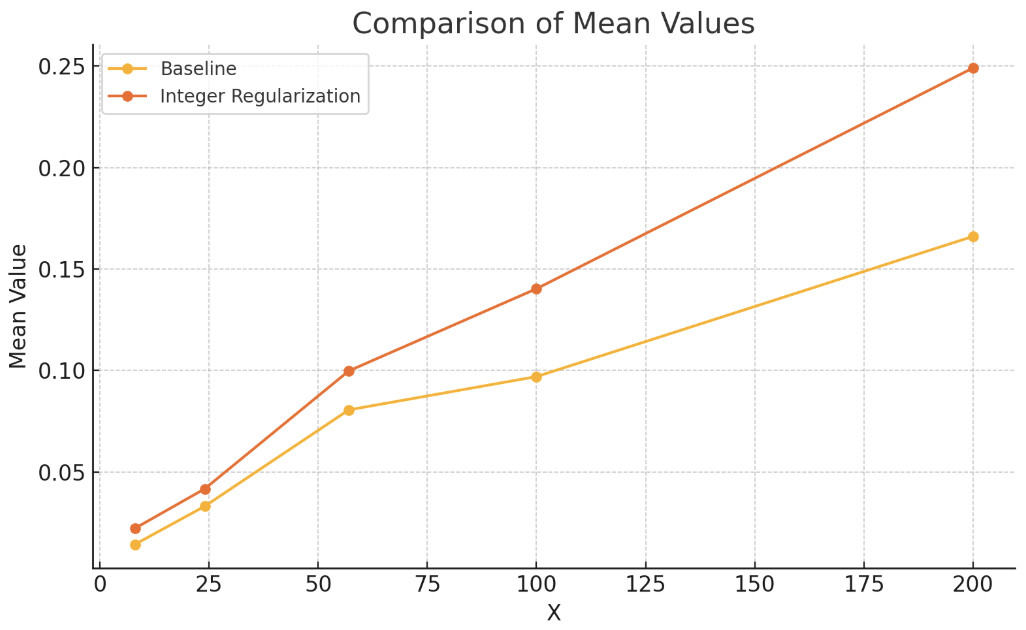
\includegraphics[width=0.5\textwidth]{images/time_comparison}
    \caption{Mean time comparison with and without using integer regularization. Increasing linearly as seen in Table \ref{tab:time}}
    \label{fig:time_comparison}
\end{figure}

\begin{table}[H]
    \centering
    \begin{tabular}{lcc}
        \textbf{Features} & \textbf{\ding{55} Integer} & \textbf{\ding{51} Integer}\\
        % \textbf{Features} & \textbf{✗ Integer} & \textbf{✓ Integer}\\
        \midrule
        8  & $6.1818$ & $8.9886$\\
        24 & $6.9653$ & $9.9545$\\
        \midrule
        57 & $10.3594$ & $11.0595$\\
        \midrule
        100 & $4.4674$ & $6.2065$\\
        200 & $4.7283$ & $6.4783$\\
        \bottomrule
    \end{tabular}
    \caption{Average epochs taken to output a counterfactual, over 176 runs, as a function of the number of features. Results shown without integer regularization(\ding{55}) and with integer regularization(\ding{51}). Numbers show that the number of epochs are dataset depending.}\label{tab:epochs}
\end{table}

Table~\ref{tab:time} shows that the time grows almost linearly with the dimensionality of the search space: increasing the number of features from~$8$ to~$200$, a $25\times$ jump, multiplies the average run-time by only $11.6\times$ ($0.014\,$s $\rightarrow 0.166\,$s). The small standard deviations confirm that these averages are representative across the $176$ test instances.

Adding the integer regularization increases the runtime in $\approx 30\text{-}50\%$ throughout the data. This extra time is spent on the additional epochs taken to apply the integer regularizer explained in Section~\ref{sec:discrete}. Even in the extreme $d=200$ case, the full version still delivers a counterfactual in well under a third of a second, keeping the
method responsive for interactive use.

It is important to note that the experiments with $8$ and $24$ features come from the loan dataset~\cite{kaggleLoan1}, the $57$-feature point corresponds to the Spambase dataset ~\cite{spambase}, and the $100$ and $200$ settings belong to the Santander Customer Transaction Prediction dataset ~\cite{santander}. This explains the relatively big change in the average epochs from $100$-$200$ epochs to $8$-$24$ epochs: the dataset makes a difference in the number of epochs needed to reach the optimal solution. As we mentioned in Section~\ref{sec:obtaining_counterfactuals}, the threshold for using the alternative update step is dataset dependent, and therefore, the number of epochs needed to reach the optimal solution is also dataset dependent. For the 100 and 200 features, a smaller threshold was used (0.2 for ~\cite{kaggleLoan1}, 0.1 for ~\cite{spambase}, and 0.05 for ~\cite{santander}), which explains the smaller number of epochs needed to reach the optimal solution. 

Across all settings, the optimizer finds a feasible solution in $4$-$11$ epochs, far below the conservative limit of $100$.  Integer regularization increases the count by roughly two epochs on average, but the absolute numbers remain very small (Figure~\ref{fig:time_comparison} illustrates the resulting trade-off). 

\subsection{Stability}\label{sec:stability}
Stability evaluates how sensitively our explainer reacts to small variations in the input. Formally ~\cite{bodria2023benchmarking}, given a counterfactual method, the metric measures the average of the maximum distances between the counterfactual generated for an instance $\mathbf{x}$ and those generated for every instance in its neighborhood ($z \in \mathcal{N}_x$). If often very similar instances receive vastly different counterfactual explanations, the explainer is deemed \textit{unstable}. In contrast, a value close to~$1$ means that the method generates similar counterfactuals for nearby points, signaling stability. The formula used to calculate the stability is the following.
\[
    \frac{1}{N} \cdot \sum_x \max_{z \in \mathcal{N}_x} \frac{\|e_x - e_{z}\|}{\|x - z\|}.
\]

\begin{table}[H]
    \centering
    \begin{tabular}{lcc}
        \textbf{Features} & \textbf{\ding{55} Integer} & \textbf{\ding{51} Integer}\\
        % \textbf{Features} & \textbf{✗ Integer} & \textbf{✓ Integer}\\
        \midrule
        loan~\cite{kaggleLoan1}  & $0.9414 \pm 0.0318$ & $2.5196 \pm 1.7558$\\
        spam~\cite{spambase} & $0.7968 \pm 0.1320$ & $0.8119 \pm 0.1326$\\
        santander~\cite{santander} & $0.9948 \pm 0.0072$ & $0.9951 \pm 0.0068$\\
        \bottomrule
    \end{tabular}
    \caption{Reports the average stability (and its standard deviation) obtained with our neural-network explainer on the three used benchmark datasets over 176 instances. The integer column correspond to calculating the metric using the integer regularizer described in Section~\ref{sec:discrete} and detailed in \autoref{alg:newton_counterfactual}.}
\end{table}

\paragraph{Loan dataset.}
Without integer constraints the explainer is already stable ($0.94\pm0.03$), yet activating the discrete regularizer more than doubles the score to $2.52$ on average.  This dataset has a lot of integer features, so it explains the big difference in stability.

\paragraph{Spam.}
E-mail features are mostly continuous TF–IDF weights, so enforcing integrality has virtually no effect ($0.7968 \pm 0.1320$ \& $0.8119 \pm 0.1326$). The relatively low absolute figures indicate that slight textual changes (such as the addition or removal of a word) has very little effects on the counterfactual proposed.

\paragraph{Santander.} Both variants achieve near-perfect stability ($\approx0.995$ with deviations $<\!0.01$), confirming that the carefully engineered numeric features already impose strong local smoothness. Discrete regularization has no effect, as all attributes are continuous.

Overall, the numbers confirm that the stability metric is dataset dependent. The little change in the stability for the Spam and Santander datasets and the big change in the Loan one suggests that the integer regularizer is much more unstable than the base counterfactual explainer, but overall it is fairly stable. Combined with the efficiency improvements reported in Section~\ref{sec:efficiency}, these results confirm that the algorithm is both \emph{fast}, \emph{scalable} and \emph{stable}, making it well suited for real-time recourse in practical applications.

\subsection{Actionability} \label{sec:actionability}
Like plausibility, actionability is not a well defined metric in the literature either. Actionability is defined as the property of a counterfactual explanation that measures whether the counterfactual can be acted upon by the user~\cite{guidotti2024counterfactual}. Like every explainer, this is one of the most important properties after validity, as the end user is the one that will act according to the counterfactual explanation. 

One of the most important requisites for a counterfactual to be actionable is that the features that are changed are actually changeable by the user. For example, if we are trying to explain a loan application, the features that are changed should be those that the user can actually change; such as income, the amount of debt, etc. No counterfactual explanation should change features that are not changeable by the user; such as his/her race, sex, etc. This poses no problem for our method, as we can select the features that we want to change in the counterfactual explanation by \emph{deactivating} the features that we do not want to change in the weight vector. 

Another important aspect of actionability is being able to generate counterfactuals that are capable of yielding integer values for discrete features. For example, a loan term feature or the number of credit lines cannot take decimal values, so the counterfactual explanation should generate integer values for those features. In our method, we can enforce this by using the regularizer explained in Section~\ref{sec:discrete}, which penalizes the distance function for discrete features and ensures that the counterfactuals generated will have integer values for those features by rounding them to the closest integer when the optimization process is close to the optimal solution.

In other papers, as well as using the common definition of actionability, they have provided more extensive definitions and metrics for this property. One of the most mentioned is aligned with the diversity property~\cite{dice}. If a counterfactual method is able to generate multiple counterfactuals that are all valid and actionable, then it is considered to be more actionable than a method that can only generate one counterfactual. This is because the user can choose the counterfactual that is most suitable for their needs, and therefore the method is more flexible and adaptable to the user's needs. 

Many methods in the literature are able to generate multiple counterfactuals with the  solution they provide. In our case, as we are solving an optimization problem, only one counterfactual is generated for a given instance and set of weights. However, by changing the weights, we can generate multiple counterfactuals that are all valid and actionable by the original definition. Other methods in the literature are able to generate multiple counterfactuals by using a diversity metric, but we have revolutionized the definition of diversity and actionability at the same time. 

Not only are we able to generate multiple counterfactuals, but we are able to generate the most suited counterfactual for the user, as they are able to specify which features are easier to change than others. This, aligned with the fulfillment of the similarity property, makes our method one of the most actionable methods in the literature following this actionability criteria. If an actionable counterfactual exists, meaning that the user is able to make the changes proposed; our method will find it by having an interactive and iterative back-and-forth \emph{dialogue} with the user.

Other definitions of actionability include the availability or success-within-budget, introduced in ~\cite{ustun2019actionable}. This paper defines the metric as the amount of counterfactuals that have a cost lower than a certain threshold. As we have mentioned, our method is able to find the minimum cost counterfactual, and because the metric is budget-dependent, we are able to fulfill it depending on the budget set. If the \emph{budget of change} is too low, the method will not be able to find an actionable counterfactual (by this definition), because it does not exist.

% \textcolor{red}{Mejora el comentario de la tabla, explicando qué se está viendo}

\begin{table}[ht]
    \centering
    \begin{tabular}{cc|ccc}
             &                 & \multicolumn{3}{c}{$w_{\text{Loan}}$} \\
     & & 0.1 & 1 & 10 \\
     \cmidrule(l){1-5}
    \multirow{3}{*}{$w_{\text{Inc}}$}
             & 0.1 & +11.14\% & +18.09\% & +19.29\% \\
             & 1   &  +2.30\% & +11.14\% & +18.09\% \\
             & 10  &  +0.24\% &  +2.28\% & +11.14\% \\
    \bottomrule
\end{tabular}

    \caption{Percentage change in Income varying weights. Similar values for proportional pairs of weights show that they are not absolute, but relative.}
    \label{tab:delta_income}
\end{table}
    
\begin{table}[ht]
    \centering
    \begin{tabular}{cc|ccc}
             &                 & \multicolumn{3}{c}{$w_{\text{Loan}}$} \\
     & & 0.1 & 1 & 10 \\
     \cmidrule(l){1-5}
    \multirow{3}{*}{$w_{\text{Inc}}$}
            & 0.1 & $-11.40$\% &  $-1.85$\% &  $-0.19$\% \\
            & 1   & $-23.53$\% & $-11.39$\% &  $-1.84$\% \\
            & 10  & $-26.34$\% & $-23.55$\% & $-11.39$\% \\
    \bottomrule
\end{tabular}

    \caption{Percentage change in LoanAmount varying weights. Values corrrespond to the table above, as when the change in income is really big ($\sim20\%$), the change in LoanAmount is small ($\sim0\%$)}
    \label{tab:delta_loan}
\end{table}

In \autoref{tab:delta_income} and \autoref{tab:delta_loan} present examples of the personalization that can be achieved with weight changes. We can see how the percentage change in the Income and LoanAmount features changes depending on the weights of their respective features in the Loan Dataset~\cite{kaggleLoan1}. The first column is the weight of the Income feature, and the first row is the weight of the LoanAmount feature. We can see that when we increase the weight of the Income feature, the percentage change in the Income feature increases, while the percentage change in the LoanAmount feature decreases. 0.1 and 10 are the minimum and maximum weights we have decided but if needed we could increase the range of weights to see how the percentage change in the features changes. 

We can also see that the percentage changes are very similar for proportional weights, meaning that the weights are not absolute and they work relative to each other. It is important to note that the values for the weights presented in the tables are not the only ones that can be used, but they are the ones that we have used for the experiments. The rest of the weights are set to 1 for these experiments.

\section{Website}\label{sec:website}
To finally ground the algorithm in a real-world application, we have used the ~\cite{kaggleLoan1} dataset to create a simple interactive web application that allows users to input their data and obtain counterfactual explanations. The web application is built using \texttt{streamlit}, a python library that allows to create interactive web applications easily. This is only an example, the website is designed to by easily adaptable to any dataset which has been cleaned and preprocessed. 

As shown in \autoref{fig:website}, the user can input their data in the form, select the features they want to change (or that they \emph{can} change), and the weights of those features. The weights are between $-1$ and $1$, but this done like this for a smoother and more intuitive user experience. In reality we take the $log_{10}$ of the value displayed. The minimum value is 0.1 and the maximum value is 10 as mentioned earlier, but this can be adjustable to any value. 
%\textcolor{red}{Explicarlo mejor que es esto de can select the value}
Categorical fields are one-hot encoded, and the user can select the value with a drop-down list. Returning to \autoref{fig:website}, we can see that the \emph{changeable} toggle button allows the user to select which features they want to change and the \emph{weights} slider allows the user to select the importance of each feature in the counterfactual explanation. These is not the case for every feature, and the entity can select which features they want the user to be able to change (for example, age is not a changeable value). The categorical features are deactivated as well, as we do not yet support the optimization of these features in the algorithm. We have as well added two buttons to showcase the website and fill the values of the form with a sample instances from the dataset, representing both classes.

\begin{figure}[H]
    \centering
    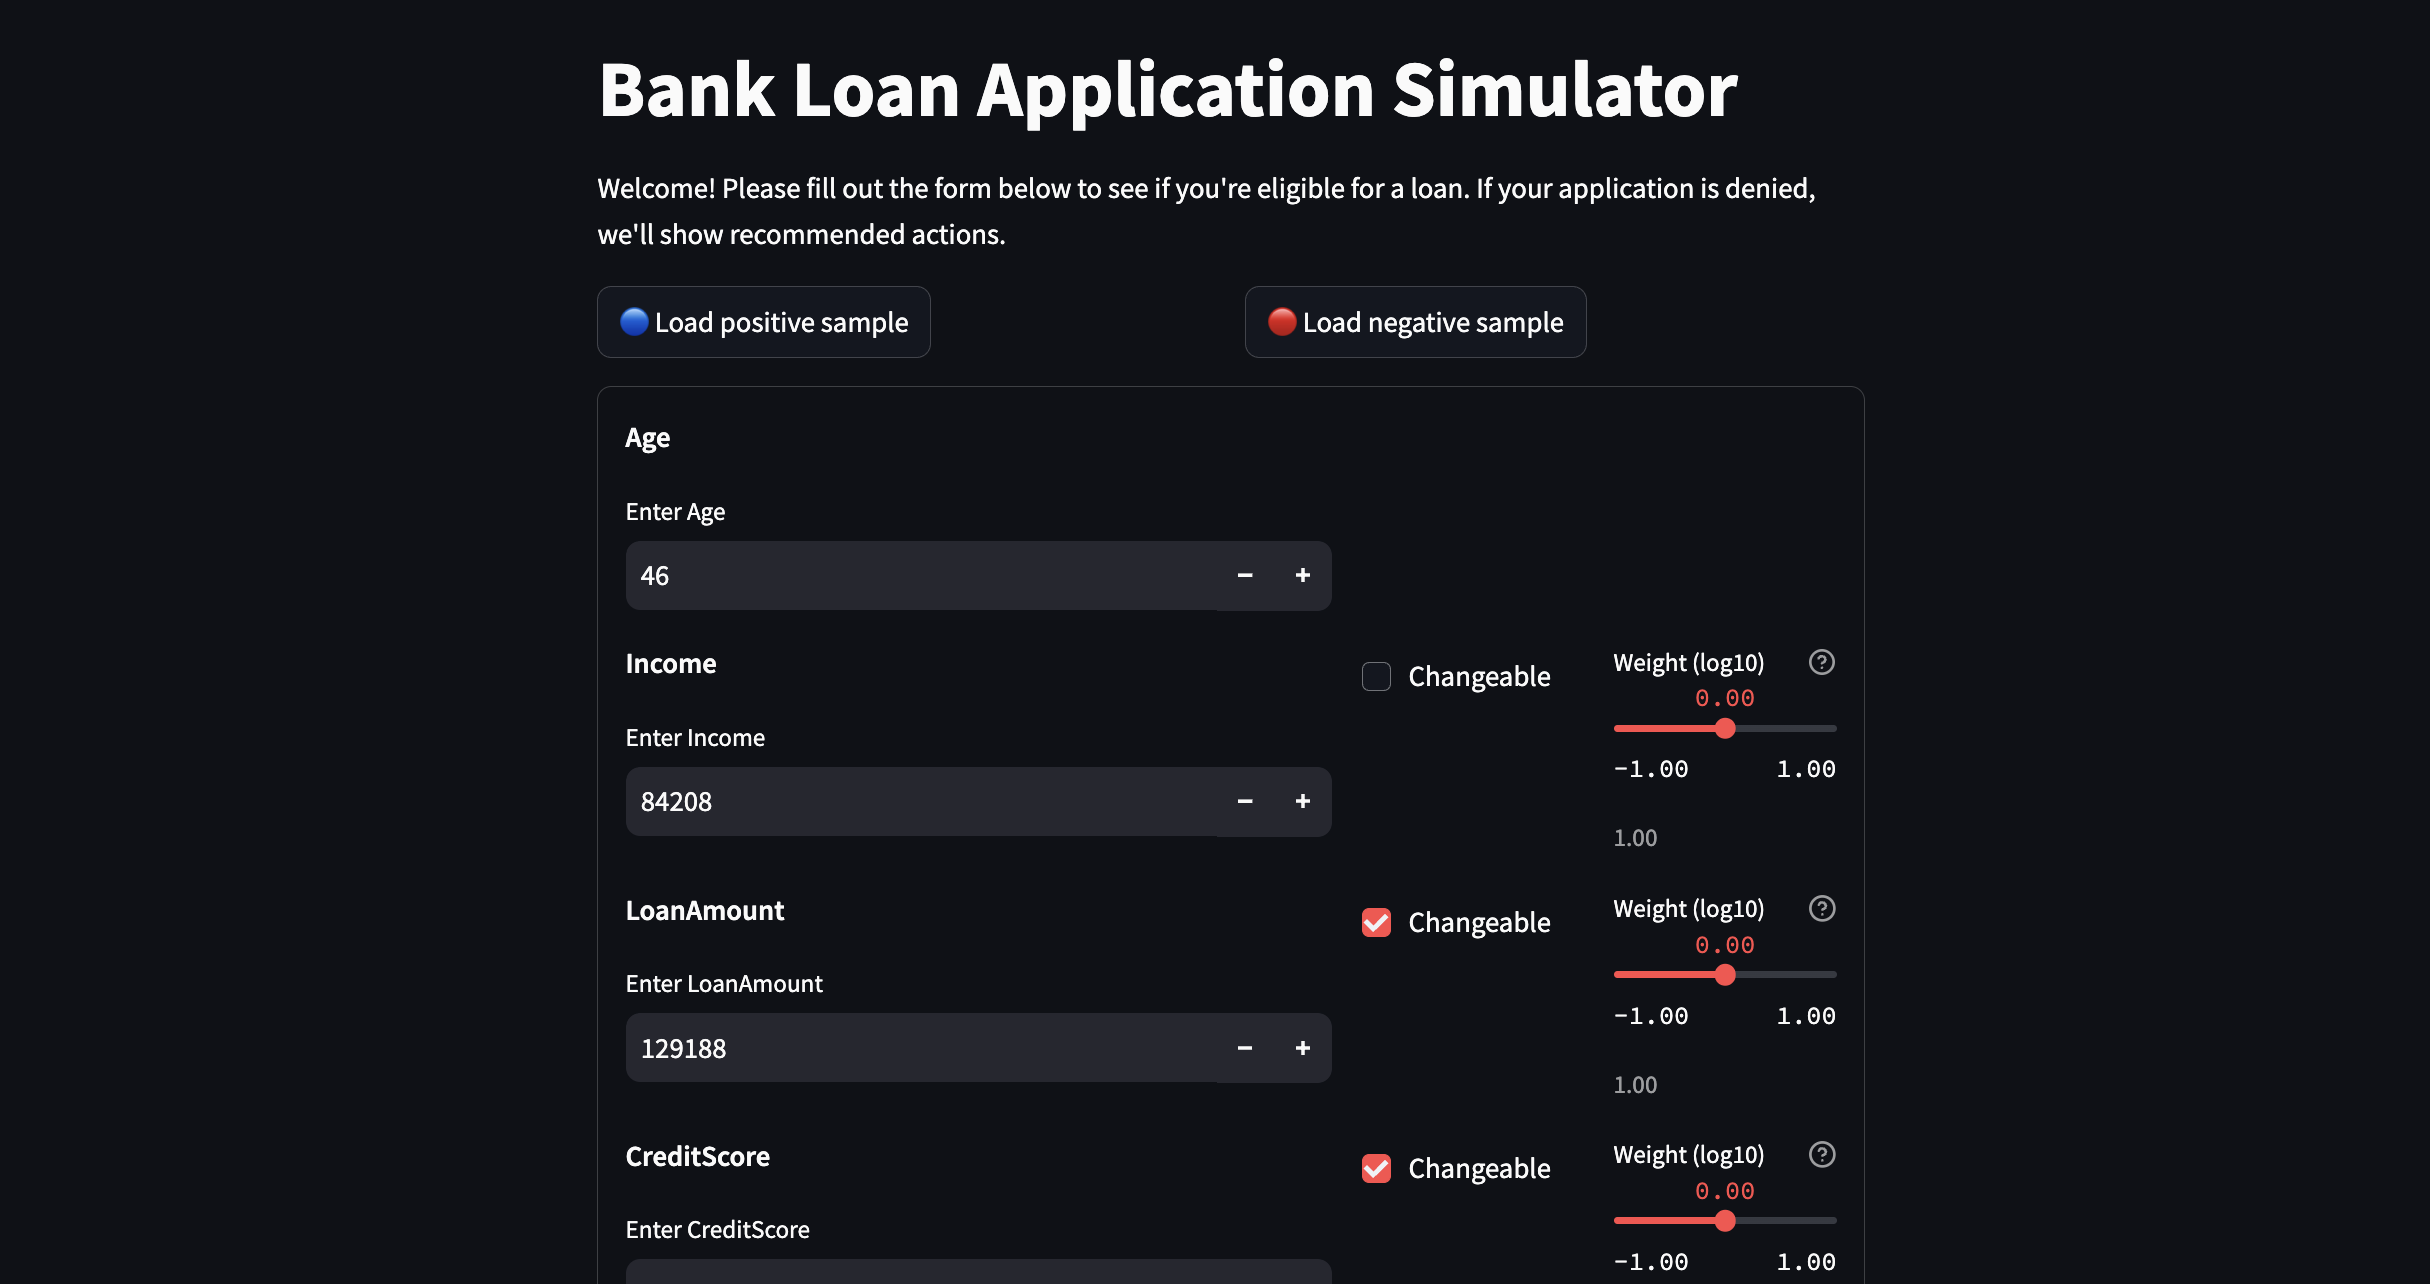
\includegraphics[width=0.8\textwidth]{images/website}
    \caption{Implementation of the algorithm in a web application using streamlit. User can determine if a field is changeable with the checkbox, and how difficult it is to change it using the slider.}
    \label{fig:website}
\end{figure}



\begin{figure}[H]
    \centering
    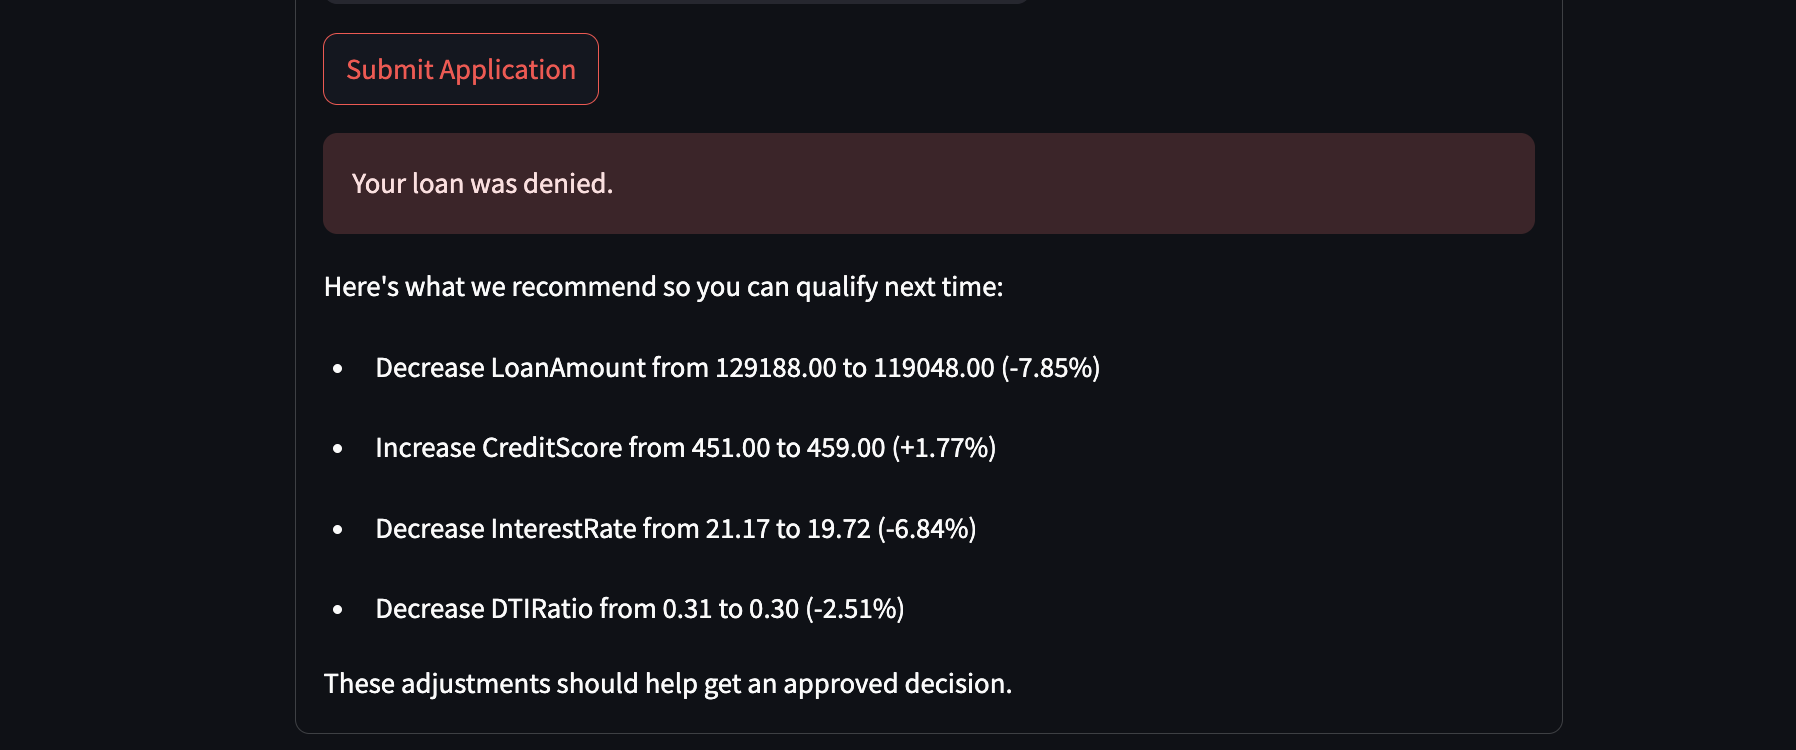
\includegraphics[width=1\textwidth]{images/website_output_denied}
    \caption{Example output of a sample classified as denied. Counterfactual provided with the percentage of change in each variable after clicking the Submit Application button.}
    \label{fig:website_output_denied}
\end{figure}
\begin{figure}[H]
    \centering
    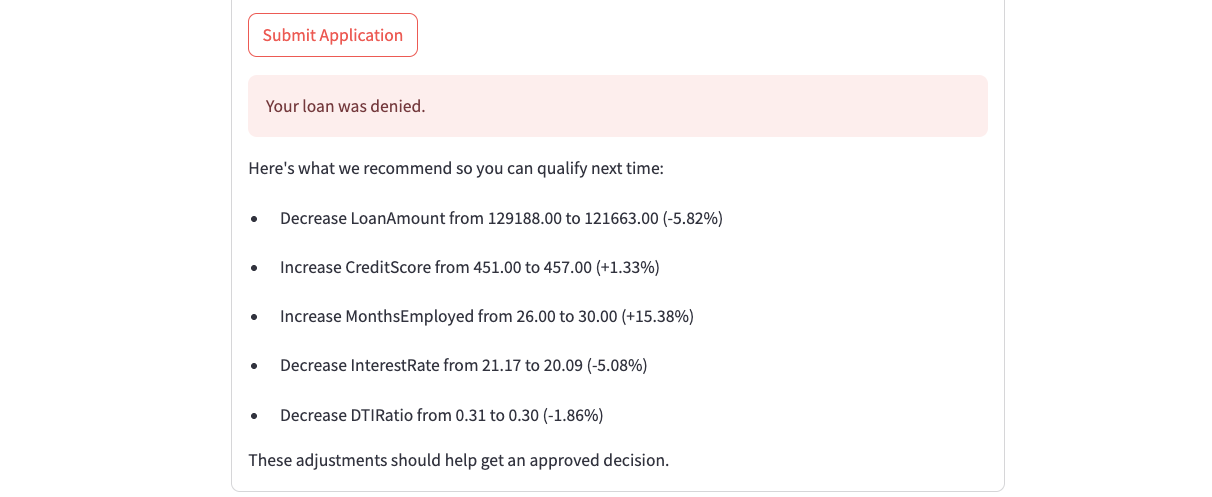
\includegraphics[width=1\textwidth]{images/website_output_approved}
    \caption{Example output of a sample classified as approved. Submitted form with values that the model classifies as positive.}
    \label{fig:website_output_approved}
\end{figure}

% \textcolor{red}{Mete más explicación a los comentarios de las figuras, explica que estás viendo en cada imagen, que es importante de cada imagen, ...}

When the user clicks on the \emph{Submit Application} button, the model generates a prediction for that instance, and, if the application is denied; the algorithm is run to find a counterfactual explanation. The output is shown in \autoref{fig:website_output_denied}, where it shows the output of the algorithm, which is the counterfactual explanation. Here, it shows the original value and the minimal changes that have to happen to each individual feature to change the classification output of the model. If we were to change each feature to the value shown, the model would classify the instance as approved and return what we see in \autoref{fig:website_output_approved}.


\section{Conclusions and Future Work}\label{sec:conclusion}

This paper introduces the first counterfactual-explanation algorithm fully grounded in Newton optimization.  
By using second derivatives, the method converges in only a handful of iterations to the \emph{minimum} perturbation that flips the decision of any differentiable classifier (e.g.,\ neural networks, logistic regressions).  

We are also the first to incorporate an explicit \emph{weight vector} in the cost function, encoding the real-world difficulty of changing a feature directly into the optimization objective. This simple yet powerful mechanism allows end-users to steer the explanation toward truly actionable recommendations.

The \texttt{PyTorch} code is written as a modular library: it works on any tabular dataset but can be tailored to organization-specific rules with a few lines of configuration. Typical customizations could include the creation of granular continuous features, enforcing that a variable changes with a specific step size (e.g. salary changes only come in \(\,\$5\,000\) or that the loan term can only be expressed in whole years). As we mentioned before, the entity can also select which features appear changeable and which are not (e.g. the interest rates are set by themselves, or they are not changeable by the user).

The combination of weighted controllability, flexible feature handling and Newton's rapid convergence yields counterfactuals that are valid, minimal, plausible, efficient, stable, and immediately actionable, while keeping runtime under a quarter of a second for datasets with up to 200 features. Because the optimizer is model-agnostic and the weighting scheme encodes domain knowledge directly, the approach is ready for deployment in highly regulated settings such as credit approval.
% \textbf{Nominal categories}: each one-hot group is relaxed to a probability simplex, regularized entropically to stay near the simplex vertices, and finally “snapped’’ to the highest-probability category at convergence.

In the future, we would extend the algorithm to ensure some kind of minimality with respect to the features, adding a regularizer that penalizes the number of features changed. There is a challenge in balancing the similarity and minimality of the method that needs to be resolved. 

We would explore the possibility of optimizing the weights of the features to provide an initial value or guess instead of starting with all weights equal to 1. We would need to record data from the users to be able to do this, by retrieving feedback from the users in order to optimize the initial set of weights based on previous interactions with the platform (of the same usar and users with a similar profile). This would allow us to provide a more personalized experience, as the algorithm would be able to learn from the user's preferences and adapt to them.

Future implementations will extend the algorithm to work with categorical features. This would allow us to provide counterfactual explanations for a wider range of datasets and use cases, making the algorithm more versatile and applicable to real-world scenarios. We have theorized how to do this with entropic regularizers. The idea is to treat each one-hot group as a probability simplex, apply an entropic regularizer to keep the vector near the vertices, and then snap to the highest-probability value at the end, similar to the approach used for discrete features. However, the implementation details remain undone.

Finally, with a strong framework created, we plan to approach companies like banks with use cases tailored to their industry, to show the potential these explanations have in their products.

\begin{thebibliography}{99}

\bibitem{wachter2017counterfactual}
S.~Wachter, B.~Mittelstadt, and C.~Russell.
\newblock Counterfactual Explanations without Opening the Black Box: Automated Decisions and the GDPR.
\newblock {\em SSRN Electronic Journal}, 2017.

\bibitem{guidotti2024counterfactual}
R.~Guidotti.
\newblock Counterfactual Explanations and How to Find Them: Literature Review and Benchmarking.
\newblock {\em Data Mining and Knowledge Discovery}, 38:2770--2824, 2024.

\bibitem{bodria2023benchmarking}
F.~Bodria, F.~Giannotti, R.~Guidotti, F.~Naretto, D.~Pedreschi, and S.~Rinzivillo.
\newblock Benchmarking and survey of explanation methods for black box models.
\newblock {\em Data Mining and Knowledge Discovery}, 37(5):1719--1778, 2023.

\bibitem{ustun2019actionable}
B.~Ustun, A.~Spangher, and Y.~Liu.
\newblock Actionable Recourse in Linear Classification.
\newblock {\em Proceedings of KDD '19}, 2019.

\bibitem{lime}
M.~T. Ribeiro, S.~Singh, and C.~Guestrin.
\newblock ``Why Should I Trust You?'': Explaining the Predictions of Any Classifier.
\newblock Proceedings of the 22nd {ACM} {SIGKDD} International Conference on
               Knowledge Discovery and Data Mining, San Francisco, CA, USA, August
               13-17, 2016

\bibitem{shap}
S.~Lundberg and S.-I. Lee.
\newblock A Unified Approach to Interpreting Model Predictions.
\newblock Advances in Neural Information Processing Systems, : Curran Associates, Inc. 2017.

\bibitem{cohen2021black}
S.~N. Cohen, D.~Snow, and L.~Szpruch.
\newblock Black-Box Model Risk in Finance.
\newblock {\em SSRN Electronic Journal}, 2021.

\bibitem{ghatasheh2014business}
N.~Ghatasheh.
\newblock Business analytics using random forest trees for credit risk prediction: a comparison study.
\newblock {\em International Journal of Advanced Science and Technology}, 72:19--30, 2014.

\bibitem{pointofview}
Anonymous.
\newblock Point of View: Using Random Forest for credit risk models (Machine learning and Credit Risk: a suitable marriage?), 2019.

\bibitem{fliege2009newton}
J.~Fliege, L.~M.~G. Drummond, and B.~F. Svaiter.
\newblock Newton's Method for Multiobjective Optimization.
\newblock {\em SIAM Journal on Optimization}, 20(2):602--626, 2009.

\bibitem{ypmanewton}
Ypma, T. J. 
\newblock Historical Development of the Newton-Raphson Method. SIAM Review, 37(4), 531–551. 
\newblock 1995.
\newblock \url{http://www.jstor.org/stable/2132904}

\bibitem{lagrange}
Bertsekas, D. P. 
\newblock Constrained Optimization and Lagrange Multiplier Methods (Optimization and Neural Computation Series).
\newblock 1996.
\newblock Athena Scientific. ISBN: 1886529043

\bibitem{papakonstantinou2009historical}
J.~M. Papakonstantinou.
\newblock Historical Development of the BFGS Secant Method and its Characterization Properties.
\newblock 2009.

\bibitem{plausibility}
Keane, M.~T., Kenny, E.~M., Delaney, E., \& Smyth, B. (2021).
\newblock \textit{If only we had better counterfactual explanations:
Five key deficits to rectify in the evaluation of counterfactual XAI techniques}.
Proceedings of the 30th International Joint Conference on Artificial
Intelligence (IJCAI-21).

\bibitem{kaggleLoan1}
\newblock H, M.~Y. (2022). Loan default dataset. Kaggle. 
\newblock \url{https://www.kaggle.com/datasets/yasserh/loan-default-dataset}.

\bibitem{spambase}
\newblock Hopkins, M., Reeber, E., Forman, G., \& Suermondt, J. (1999). Spambase [Dataset]. UCI Machine Learning Repository. .
\newblock \url{https://doi.org/10.24432/C53G6X}.

\bibitem{santander}
\newblock Piedra, M., Dane, S., \& Jimenez, S. (2019). Santander Customer Transaction Prediction [Competition]. Kaggle.
\newblock \url{https://kaggle.com/competitions/santander-customer-transaction-prediction}.

\bibitem{sgd}
H.~Robbins and S.~Monro.
\newblock A Stochastic Approximation Method.
\newblock {\em The Annals of Mathematical Statistics}, 22(3):400--407, 1951.

\bibitem{adam}
D.~P. Kingma and J.~Ba.
\newblock Adam: A Method for Stochastic Optimization.
\newblock In {\em Proceedings of the 3rd International Conference on Learning Representations (ICLR)}, 2015.

\bibitem{lof}
M.~M. Breunig, H.-P. Kriegel, R.~T. Ng, and J.~Sander.
\newblock LOF: Identifying Density-Based Local Outliers.
\newblock In {\em Proceedings of the 2000 ACM SIGMOD International Conference on Management of Data}, 2000.

\bibitem{dpprocess}
Kulesza, A. \& Taskar, B.
\newblock Determinantal Point Processes for Machine Learning.
\newblock Foundations and Trends in Machine Learning, 5, 123-286, 2012

\bibitem{limecshapc}
Y.~Ramon, D.~Martens, F.~Provost, and T.~Evgeniou.
\newblock A comparison of instance-level counterfactual explanation algorithms for behavioral and textual data: SEDC, LIME-C and SHAP-C.
\newblock {\em Advances in Data Analysis and Classification}, 14(4):801--819, 2020.

\bibitem{dice}
R.~K. Mothilal, A.~Sharma, and C.~Tan.
\newblock Explaining machine learning classifiers through diverse counterfactual explanations.
\newblock In {\em Proceedings of the 2020 Conference on Fairness, Accountability, and Transparency (FAT* '20)}, pages 607--617, 2020.

\bibitem{sgnce}
K.~Mohammadi, A.-H. Karimi, G.~Barthe, and I.~Valera.
\newblock Scaling Guarantees for Nearest Counterfactual Explanations.
\newblock In M. Fourcade, B. Kuipers, S. Lazar \& D. K. Mulligan (eds.), AIES (p./pp. 177-187), : ACM. ISBN: 978-1-4503-8473-5, 2021.

\bibitem{numopt}
Nocedal, J., Wright, S. J. (2006). Numerical optimization.
\newblock New York, NY: Springer. ISBN: 978-0-387-30303-1
 
\bibitem{scipyopt}
SciPy Development Team.
\newblock \textit{scipy.optimize.newton} (Version 1.15.3) [Computer-software documentation], 2025.
\newblock SciPy. Retrieved June 4, 2025, from \url{https://docs.scipy.org/doc/scipy/reference/generated/scipy.optimize.newton.html}.

\end{thebibliography}




\end{document}




